%%%%%%%% ICML 2025 EXAMPLE LATEX SUBMISSION FILE %%%%%%%%%%%%%%%%%

\documentclass{article}
%%%%% NEW MATH DEFINITIONS %%%%%

% \usepackage{amsmath,amsfonts,bm}
\usepackage{amsmath,amsfonts}

\usepackage{pifont}


\newcommand{\R}{\mathbb{R}}


\def\va{{\mathbf{a}}}
\def\vg{{\mathbf{g}}}

% Sets
\def\sR{\mathbb{R}}
\def\sC{\mathbb{C}}
\def\sZ{\mathbb{Z}}
\def\sN{\mathbb{N}}
\def\sQ{\mathbb{Q}}

\def\sS{\mathcal{S}}



% Vectors
\def\vzero{{\mathbf{0}}}
\def\vone{{\mathbf{1}}}
\def\vmu{{\mathbf{\mu}}}
\def\vtheta{{\mathbf{\theta}}}
\def\va{{\mathbf{a}}}
\def\vb{{\mathbf{b}}}
\def\vc{{\mathbf{c}}}
\def\vd{{\mathbf{d}}}
\def\ve{{\mathbf{e}}}
\def\vf{{\mathbf{f}}}
\def\vg{{\mathbf{g}}}
\def\vh{{\mathbf{h}}}
\def\vi{{\mathbf{i}}}
\def\vj{{\mathbf{j}}}
\def\vk{{\mathbf{k}}}
\def\vl{{\mathbf{l}}}
\def\vm{{\mathbf{m}}}
\def\vn{{\mathbf{n}}}
\def\vo{{\mathbf{o}}}
\def\vp{{\mathbf{p}}}
\def\vq{{\mathbf{q}}}
\def\vr{{\mathbf{r}}}
\def\vs{{\mathbf{s}}}
\def\vt{{\mathbf{t}}}
\def\vu{{\mathbf{u}}}
\def\vv{{\mathbf{v}}}
\def\vw{{\mathbf{w}}}
\def\vx{{\mathbf{x}}}
\def\vy{{\mathbf{y}}}
\def\vz{{\mathbf{z}}}
\def\vzeta{{\mathbf{\zeta}}}

% Matrix
\def\mA{{\mathbf{A}}}
\def\mB{{\mathbf{B}}}
\def\mC{{\mathbf{C}}}
\def\mD{{\mathbf{D}}}
\def\mE{{\mathbf{E}}}
\def\mF{{\mathbf{F}}}
\def\mG{{\mathbf{G}}}
\def\mH{{\mathbf{H}}}
\def\mI{{\mathbf{I}}}
\def\mJ{{\mathbf{J}}}
\def\mK{{\mathbf{K}}}
\def\mL{{\mathbf{L}}}
\def\mM{{\mathbf{M}}}
\def\mN{{\mathbf{N}}}
\def\mO{{\mathbf{O}}}
\def\mP{{\mathbf{P}}}
\def\mQ{{\mathbf{Q}}}
\def\mR{{\mathbf{R}}}
\def\mS{{\mathbf{S}}}
\def\mT{{\mathbf{T}}}
\def\mU{{\mathbf{U}}}
\def\mV{{\mathbf{V}}}
\def\mW{{\mathbf{W}}}
\def\mX{{\mathbf{X}}}
\def\mY{{\mathbf{Y}}}
\def\mZ{{\mathbf{Z}}}
\def\mBeta{{\mathbf{\beta}}}
\def\mPhi{{\mathbf{\Phi}}}
\def\mLambda{{\mathbf{\Lambda}}}
\def\mSigma{{\mathbf{\Sigma}}}


% Expectation
% \def\eE{\mathop{\mathbb{E}}\limits}
\def\eE{\mathbb{E}}

% Probability
\def\pP{\mathbb{P}}

% Tilde
\def\tf{\tilde{f}}
\def\tS{\tilde{S}}
\def\wtF{\widetilde{\mathcal{F}}}
\def\whR{\widehat{R}}
\def\tvx{\tilde{\mathbf{x}}}
\def\ty{\tilde{y}}


\def\defeq{\overset{\textup{def}}{=}}
% \def\defeq{\overset{.}{=}}
\def\defone{\overset{\text{\ding{172}}}{=}}
\def\deftwo{\overset{\text{\ding{173}}}{=}}
\def\leqone{\overset{\text{\ding{172}}}{\leq}}
\def\leqtwo{\overset{\text{\ding{173}}}{\leq}}
\def\leqthree{\overset{\text{\ding{174}}}{\leq}}
\def\leqfour{\overset{\text{\ding{175}}}{\leq}}
\def\eqone{\overset{\text{\ding{172}}}{=}}
\def\eqtwo{\overset{\text{\ding{173}}}{=}}
\def\eqthree{\overset{\text{\ding{174}}}{=}}
\def\eqfour{\overset{\text{\ding{175}}}{=}}
\def\geqfive{\overset{\text{\ding{176}}}{\geq}}

\usepackage{url}
\usepackage{footmisc}
\usepackage{caption}
\usepackage{subcaption}
\usepackage{xcolor}
\usepackage{tikz}

\usepackage{color}
\usetikzlibrary{positioning, arrows, automata}
\usetikzlibrary{backgrounds, calc}
\usepackage{pgfplots}
\pgfplotsset{compat=1.8}
\usepackage{pgfplotstable}
\usepgfplotslibrary{groupplots}

% Recommended, but optional, packages for figures and better typesetting:
\usepackage{microtype}
\usepackage{graphicx}
\usepackage{booktabs} % for professional tables

% hyperref makes hyperlinks in the resulting PDF.
% If your build breaks (sometimes temporarily if a hyperlink spans a page)
% please comment out the following usepackage line and replace
% \usepackage{icml2025} with \usepackage[nohyperref]{icml2025} above.
\usepackage{hyperref}


% Attempt to make hyperref and algorithmic work together better:
\newcommand{\theHalgorithm}{\arabic{algorithm}}

% Use the following line for the initial blind version submitted for review:
% \usepackage{icml2025}

% If accepted, instead use the following line for the camera-ready submission:
\usepackage[accepted]{icml2025}

% For theorems and such
\usepackage{amsmath}
\usepackage{amssymb}
\usepackage{mathtools}
\usepackage{amsthm}

% Colors used for tikz plotting
\usetikzlibrary{positioning, arrows, automata, matrix}

\usepgfplotslibrary{groupplots}
\usepgfplotslibrary{colorbrewer}
\usetikzlibrary{external}
\usetikzlibrary{backgrounds, calc}
\usetikzlibrary{spy}
\usetikzlibrary{fit}
\usetikzlibrary{arrows.meta}
\usepackage{adjustbox}
\usepackage{graphicx}

% Util colors and thickness for plotting
\definecolor{lightgray204}{RGB}{204,204,204}
\definecolor{plot_background}{HTML}{EBF0F0}
\def\linewidthdime{1mm}
\def\linewidthother{0.5mm}

%
% Color-Method Mapping, e.g. C1 is for Bro
%
\definecolor{C0}{HTML}{1f77b4}  % Blue, DIME
\definecolor{C1}{HTML}{ff7f0e}  % Orange, BRO
\definecolor{C2}{HTML}{2ca02c}  % Green, CrossQ
\definecolor{C3}{HTML}{d62728}  % Red, QSM
\definecolor{C4}{HTML}{9467bd}  % Purple, Diff-QL
\definecolor{C5}{HTML}{8c564b}  % Brown, Consinstency-AC
\definecolor{C6}{HTML}{e377c2}  % Pink, DIPO
%===================================================
\definecolor{C7}{HTML}{7f7f7f}  % Gray,
\definecolor{C8}{HTML}{bcbd22}  % Yellow Green, 
\definecolor{C9}{HTML}{17becf}  % Cyan,
\definecolor{C10}{HTML}{CCCC00} % Yellow,

% if you use cleveref..
\usepackage[capitalize,noabbrev]{cleveref}

\newcommand{\fpi}{\vec{\pi}}
\newcommand{\bpi}{\cev{\pi}}
\newcommand{\bq}{\cev{q}}
\newcommand{\ppi}{\pi^{\theta}}

\newcommand{\ac}{a}
\newcommand{\st}{s}
\newcommand{\dQ}{Q_{\text{D}}}
\newcommand{\dV}{V_{\text{D}}}
\newcommand{\dpi}{\pi_{\text{D}}}
\newcommand{\St}{\mathcal{S}}
\newcommand{\Ac}{\mathcal{A}}
\newcommand{\Ent}{\mathcal{H}}
\newcommand{\Z}{\mathcal{Z}}
\newcommand{\fP}{\vec{\mathbb{P}}}
\newcommand{\bP}{\cev{\mathbb{P}}}
\newcommand{\plb}{\ell^{\theta}_{\mathcal{H}}}
\newcommand{\lb}{\ell^{\theta}_{\mathcal{H}}}
\definecolor{nfvi}{RGB}{255,127,14} % orange
\newcommand{\baseline}[1]{\textcolor{nfvi}{#1}}
\newcommand{\blb}{\ell_{\bpi}}

%%%%%%%%%%%%%%%%%%%%%%%%%%%%%%%%
% THEOREMS
%%%%%%%%%%%%%%%%%%%%%%%%%%%%%%%%
\theoremstyle{plain}
\newtheorem{theorem}{Theorem}[section]
\newtheorem{proposition}[theorem]{Proposition}
\newtheorem{lemma}[theorem]{Lemma}
\newtheorem{corollary}[theorem]{Corollary}
\theoremstyle{definition}
\newtheorem{definition}[theorem]{Definition}
\newtheorem{assumption}[theorem]{Assumption}
\theoremstyle{remark}
\newtheorem{remark}[theorem]{Remark}

% Todonotes is useful during development; simply uncomment the next line
%    and comment out the line below the next line to turn off comments
\usepackage[disable,textsize=tiny]{todonotes}
%\usepackage[textsize=tiny]{todonotes}


% The \icmltitle you define below is probably too long as a header.
% Therefore, a short form for the running title is supplied here:
\icmltitlerunning{DIME: Diffusion-Based Maximum Entropy Reinforcement Learning}

\begin{document}

\twocolumn[
\icmltitle{DIME: Diffusion-Based Maximum Entropy Reinforcement Learning}

% It is OKAY to include author information, even for blind
% submissions: the style file will automatically remove it for you
% unless you've provided the [accepted] option to the icml2025
% package.

% List of affiliations: The first argument should be a (short)
% identifier you will use later to specify author affiliations
% Academic affiliations should list Department, University, City, Region, Country
% Industry affiliations should list Company, City, Region, Country

% You can specify symbols, otherwise they are numbered in order.
% Ideally, you should not use this facility. Affiliations will be numbered
% in order of appearance and this is the preferred way.
\icmlsetsymbol{equal}{*}
% Onur Celik, Zechu Li, Denis Blessing, Ge Li, Daniel Palenicek, Jan Peters, Georgia Chalvatzaki, Gerhard Neumann
\begin{icmlauthorlist}
\icmlauthor{Onur Celik}{kit}
\icmlauthor{Zechu Li}{tud}
\icmlauthor{Denis Blessing}{kit}
\icmlauthor{Ge Li}{kit}
\icmlauthor{Daniel Palenicek}{tud,hessianai}\\
\icmlauthor{Jan Peters}{tud,hessianai,dfki,cogscience}
\icmlauthor{Georgia Chalvatzaki}{tud,hessianai}
\icmlauthor{Gerhard Neumann}{kit}
\end{icmlauthorlist}

\icmlaffiliation{kit}{Karlsruhe Institute of Technology, Germany}
\icmlaffiliation{tud}{Technical University of Darmstadt, Germany}
\icmlaffiliation{hessianai}{Hessian.AI}
\icmlaffiliation{dfki}{German Research Center for AI(DFKI)}
\icmlaffiliation{cogscience}{Centre for Cognitive Science, TU Darmstadt}
% \icmlaffiliation{sch}{School of ZZZ, Institute of WWW, Location, Country}

\icmlcorrespondingauthor{Onur Celik}{celik@kit.edu}
% \icmlcorrespondingauthor{Firstname2 Lastname2}{first2.last2@www.uk}

% You may provide any keywords that you
% find helpful for describing your paper; these are used to populate
% the "keywords" metadata in the PDF but will not be shown in the document
\icmlkeywords{Machine Learning}

\vskip 0.3in
]

% this must go after the closing bracket ] following \twocolumn[ ...

% This command actually creates the footnote in the first column
% listing the affiliations and the copyright notice.
% The command takes one argument, which is text to display at the start of the footnote.
% The \icmlEqualContribution command is standard text for equal contribution.
% Remove it (just {}) if you do not need this facility.

%\printAffiliationsAndNotice{}  % leave blank if no need to mention equal contribution
\printAffiliationsAndNotice{\icmlEqualContribution} % otherwise use the standard text.
\begin{abstract}
Maximum entropy reinforcement learning (MaxEnt-RL) 
has become the standard approach to RL due to its beneficial exploration properties. Traditionally, policies are parameterized using Gaussian distributions, which significantly limits their representational capacity. Diffusion-based policies offer a more expressive alternative, yet integrating them into MaxEnt-RL poses challenges—primarily due to the intractability of computing their marginal entropy. 
To overcome this, we propose Diffusion-Based Maximum Entropy RL (DIME). \emph{DIME} leverages recent advances in approximate inference with diffusion models to derive a lower bound on the maximum entropy objective. 
Additionally, we propose a policy iteration scheme that provably converges to the optimal diffusion policy. Our method enables the use of expressive diffusion-based policies while retaining the principled exploration benefits of MaxEnt-RL, significantly outperforming other diffusion-based methods on challenging high-dimensional control benchmarks. It is also competitive with state-of-the-art non-diffusion based RL methods while requiring fewer algorithmic design choices and smaller update-to-data ratios, reducing computational complexity.  
\end{abstract}


\documentclass[../main.tex]{subfiles}
\graphicspath{{../images/}}
\makeatletter
\def\input@path{{../images/}}
\makeatother
\begin{document}
\section{Introduction}
\begin{figure}
\centering
\begin{tikzpicture}
\node[inner sep=0pt] (ws) at (0, 0) {
\includegraphics[height=.4\textwidth, trim={10cm 0 10cm 0},clip]{world_space.png}};
\node[inner sep=0pt] (cs) at (6,0) {\includegraphics[height=.4\textwidth, trim={10cm 1cm 10cm 4cm},clip]{conf_space.png}};
\end{tikzpicture}
\vspace{-5pt}
\label{fig:pbrm_intro}
\caption{\textbf{Left}: Shows world space obstacles as grey spheres. Robots start and goal configuration is colored red and green, respectively. Configurations along the computed path are colored transparent blue. \textbf{Right:} Mapped world space scenario to configuration space. Obstacle region is the grey mesh. Red spheres are collision-free regions computed by the neural SCDF. The optimized shortest path in the convex corridor is the blue curve.}
\vspace{-25pt}
\end{figure}
Motion planning is the problem of finding a collision-free trajectory that connects a given start and goal configuration. The planning takes place in the configuration space of the robot. For single body robots, like mobile robots or drones, the configuration space and the world space are usually the same. This simplifies the planning, since explicit obstacle representations are available which enables geometrical tools like separating hyperplanes, smallest distance to obstacles etc., to be used when designing motion planning algorithms. For multi-body robots like manipulators, the situation is completely different. The world space obstacles are usually mapped to non-convex regions, and to make the problem even harder, the mapping is usually not known. Forming explicit representations of the obstacle region in the configuration space is usually too expensive or intractable. Despite all of this, sampling based planners are used with great success, which mainly is due to their use of implicit representations of the obstacle region. The basic idea is to construct a graph in the configuration space that covers and connects the collision-free region. From this graph, a path can be extracted that connects a given start and goal configuration. The approach is computationally expensive, since the graph is constructed with the smallest geometrical building block available, points, which represents a collision-check. Furthermore, the extracted paths from the graph are non-smooth and jagged due to the stochastic nature of the approach. This adds an additional post-processing step to the process, where the paths are shortcutted and smoothened, before the path can be used for tracking. Clearly a lot of time is invested to form this graph and produce smooth paths. Thus, if the obstacles start to move, then all of this work is done in no use, since all points that make up this graph need to be re-verified, which is simply too time consuming to be done in real time.
\\\\
In this work, we want to address the existing drawbacks of the sampling based planners. Our main contribution is an improved motion planner where each vertex in the graph covers a collision-free region in the form of a sphere instead of a point and where the edges are formed with neighboring intersecting spheres. This representation has the advantage of instead of returning piecewise linear paths, returning a sequence of overlapping spheres, i.e. a convex corridor, that connects a given start and goal configuration, illustrated in Figure \ref{fig:pbrm_intro}. This convex corridor allows us to use convex optimization to produce smooth trajectories, instead of computationally expensive post-processing methods. The representation further allows us to estimate the coverage of the collision-free space, which gives us awareness and feedback in the offline roadmap construction phase. Finally, our representation is simple to adapt to moving obstacles, simply requery for the new radii and recheck for intersections. 
\\\\
The spherical collision-free regions are formed using a signed distance function (SDF), which is a function that returns the smallest distance from an arbitrary point to the boundary of an obstacle. As the name implies, the distance is signed, thus if the point is inside the obstacle it is negative otherwise positive. If the distance is positive, a sphere with radius equal to the distance is guaranteed to cover a collision-free region. Using an SDF in motion planning is not new, but what is novel about our approach is that we express the distance in the configuration space instead of the world space and by doing so allows us to form these convex collision-free regions. We refer to the resulting SDF as a signed configuration distance function (SCDF). Computing an SCDF analytically is non-trivial, our approach is therefore to parameterize the SCDF with a deep neural network and learn the mapping by supervised learning. Our resulting neural SCDF can compute distances for different parameter values of obstacle shapes and we also show how multiple distances can be combined, thus making our approach flexible.
\section{Related work}
Motion planning algorithms can roughly be divided into three families, grid-based, sampling based and optimization based methods. Grid-based methods (GBM) discretize the planning space from which a graph is then compiled. A standard search method is A$^\star$ \citep{a_star}, which is classified as an \textit{informed} search method, since it employs a heuristic function to speed up the search. A$^\star$ guarantees to return an optimal path at the level of discretization used. GBMs usually discretize the planning space by a regular lattice and this limits the GBMs to problems with low dimensionality due to the curse of dimensionality. Thus, GBMs are usually limited to single-body robots where the degrees of freedom (DOF) are low. To overcome the inherent scaling problem with the GBMs, stochastic methods are usually used for multi-body robots. These methods are termed as sampling-based methods (SBM) and core members within this family are the rapidly-exploring random trees (RRT) \citep{rrt} and the probabilistic roadmap (PRM) \citep{prm}. RRT grows a tree from the start configuration and explores the collision-free region in a rapid way until it is able to connect to the goal region. RRT is usually improved by bi-directional planning \citep{rrt_connect}, i.e. an additional tree is grown from the goal configuration and the trees are tested for connection after any tree has been expanded. RRT is a single-query method, thus it searches for a path from scratch each time it is queried. Contrary to this, PRM is a multi-query method, which solves for multiple queries without starting from scratch. PRM does this by creating a roadmap (graph) that covers the collision-free space as an offline step. The graph is then used to solve for multiple queries. PRMs are used in cases where the environment does not change since the extra offline step is too computationally costly and needs to be re-done if the environment is changed. In our work, we address this inherent issue by using a different roadmap representation. Our vertices in the graph cover a collision-free region in the form of spheres and we form the edges by checking for intersecting spheres. If something in the environment changes, we recompute the spheres radii and recheck the intersections, without relying on collision detection. We use a trained neural network to compute the sphere radius, therefore querying for the radius can be done fast, hence our representation enables the PRM for dynamic environments.
\\\\
In the recent decades, optimization based methods (OBM) \citep{chomp, schulman, itomp, stomp} have been introduced as an alternative to SBM for multi-body robots. Like the SBM, the OBMs scale well to higher dimensional problems and produce smoother motion. It is common to use a SDF in the optimization since it is a smooth function, thus enabling gradient-based methods. However, the standard way of expressing the SDF is in world space. The distance therefore needs to be mapped to the configuration space by the forward kinematics. This mapping makes the optimization problem a non-linear program (NLP), which is computationally expensive to solve. Recently, a different approach has been proposed. In \cite{mp_gcs} motion planning is formulated as a convex optimization problem by using the graph of convex sets framework \citep{gcs}. The underlying idea is to decompose the collision-free space into intersecting convex sets from which a convex optimization problem is formulated. In cases where an explicit representation of the obstacles in the configuration space exists, like for single-body robots, creating collision-free convex regions can be done fast \citep{iris}. For multi-body robots, this is non-trivial. Existing work does this successfully \citep{iris_nlp, iris_c} by an optimization based approach, but the methods are still too time consuming to be used in the presence of moving obstacles. Our approach is instead to use deep learning to learn an SDF expressed in the configuration space. With this, we can query for shortest distances to the collision boundary, which allows us to expand spherical regions which are collision-free. Our approach is fast and therefore enables our suggested roadmap planner to be used in dynamic environments.
\\\\
Recent research has focused on learning collision detection \citep{fk_kernel_distance, diffco, graphdistnet} by predicting the signed distance between the robot links and the surrounding obstacles in the world space. The learned SDF is used in trajectory optimization but since the distance is expressed in the world space, the problem becomes an NLP and therefore takes a long time to solve. We take a novel approach and suggest to instead express the signed distance in the configuration space. This allows us to improve the PRM at the same time as it enables convex optimization for trajectory optimization, which runs faster and is more reliable than NLP solvers. In \cite{cspf} a learned signed distance function in the configuration space is proposed similar to our approach. However, their approach is restricted to point cloud representations, while we propose to represent the obstacles as parameterized geometric shapes, e.g. spheres. Furthermore, we also show how to use our learned SCDF to improve an existing roadmap planner.
\section{Problem formulation}
A robot is located in the world space, $\W \subset \R^3 $. The unique location of the robot is given by its configuration $\q \in \C$, where $\C$ is the configuration space. The set of points covered by the robots bodies at a certain configuration is expressed as $\B(\q) \subset \W$. The robot is surrounded by $\NrObst$ obstacles $\O = \bigcup_{i=1}^{\NrObst} \O_i$, where  $\O_i \subset \W$. The representation of the obstacle in the configuration space is the set $\C\O_i = \{\q \in \C \: |\: \B(\q) \cap \O_i \neq \emptyset \}$. The obstacle space is formed as $\Co = \bigcup_{i=1}^{\NrObst} \C \O_i$. The complement is referred to as the free space, $\Cf = \C \setminus \Co$. The path planning problem is a tuple, ($\Cf$, $\qStart$, $\qGoal$), where we want to connect a query pair, consisting of a start, $\qStart$, and goal configuration, $\qGoal$, with a geometric path, $\q(s): [0, 1] \mapsto \Cf$, such that $\q(0)=\qStart$ and $\q(1)=\qGoal$, or report correctly when such a path does not exist.
\end{document}



\subsection{Plasticity in Neural Networks}
In recent years, various methods have been proposed to address plasticity loss.
Several works have focused on maintaining active units \cite{abbas2023loss, elsayed2024addressing} or re-initializing dead units \cite{sokar2023dormant, dohare2024loss}.
Other studies have explored limiting deviations from the initial statistics of model parameters \cite{kumar2023maintaining, lewandowski2023curvature, elsayed2024weight}.
Additionally, some methods rely on architectural modifications \cite{nikishin2024deep, lee2024slow, lewandowski2024plastic}.  
Plasticity loss also occurs in the reinforcement learning due to its inherent non-stationary. \citet{nikishin2022primacy} proposed resetting the model, while \citet{asadi2024resetting} suggested resetting the optimizer state. 

As noted by \citet{berariu2021study}, loss of plasticity can be divided into two distinct aspects: a decreased ability of networks to minimize training loss on new data (trainability) and a decreased ability to generalize to unseen data (generalizability).
While most previous works focused on trainability, \citet{lee2024slow} addressed generalizability loss.
They demonstrated that plasticity loss also occurs under a stationary distribution, as in a warm-start learning scenario where the model is pretrained on a subset of the training data and then fine-tuned on the full dataset.

Most existing studies have focused on only one of the following challenges: trainability, generalizability, or reinforcement learning.
However, in this study, we validate our AID method across all three aspects, demonstrating its effectiveness in each scenario.



\subsection{Activation Function}
Our AID method is a stochastic approach similar to Dropout while also functioning as an activation function.
Therefore, we aim to discuss previously proposed probabilistic activation functions.
Although the field of probabilistic activation functions has not seen extensive research, two noteworthy studies exist.
The first is the Randomized ReLU (RReLU) function, introduced in the Kaggle NDSB Competition \cite{xu2015empirical}.
The original ReLU function maps all negative values to zero, whereas RReLU maps negative values linearly based on a random slope.
During testing, negative values are mapped using the mean of the slope distribution.
Their experimental results suggest that RReLU effectively prevents overfitting.
Another example of a probabilistic activation function is DropReLU \cite{liang2021drop}.
DropReLU randomly determines whether a node's activation is processed through a ReLU function or a linear function.
The authors claim that DropReLU improves the generalization performance of neural networks.
The fundamental distinction between these probabilistic activation functions and our method lies in the generality of our approach.
Unlike simple probabilistic activation functions, our method encompasses techniques such as Dropout and ReLU, providing a more comprehensive framework.

Another related approach involves activation functions designed to address plasticity loss.
\citep{abbas2023loss} proposed the Concatenated Rectified Linear Units (CReLU), which concatenates the outputs of the standard ReLU applied to the input and its negation.
This structure prevents the occurrence of dead units, thereby improving plasticity.
Additionally, trainable activation functions have also been shown to effectively mitigate plasticity loss in reinforcement learning \citep{delfosseadaptive}.
Specifically, they introduced a trainable rational activation function that prevents value overfitting and overestimation in reinforcement learning.



\begin{figure*}[ht!]
    \centering
    \includegraphics[width=0.3\textwidth]{figures/sources/mainnet_pls_acc.pdf}
    \includegraphics[width=0.3\textwidth]{figures/sources/subnet_pls_acc.pdf}
    \includegraphics[width=0.3\textwidth]{figures/sources/warm_start_dropout.pdf}
    \caption{\textbf{Left.} Random label MNIST experiment using an 8-layer MLP. Higher dropout probabilities result in significant trainability loss. 
    \textbf{Middle.} Accuracy of the subnetworks trained on random target. Each subnetworks are sampled from original network after each epoch. Subnetworks of the Dropout also experience trainability loss. \textbf{Right.} Warm-start scenario of Resnet-18 model with CIFAR100 dataset. Dropout improves generalization performance; however, the reduction in accuracy compared to the cold-start scenario is nearly identical to that of the vanilla model.}
    \label{exp_dropout}
\end{figure*}




\section{Preliminaries}\label{sec:preliminaries}



%We denote by $(\Ac(x_\Ac),\Bc(x_\Bc))(z)$ a random execution of $\pi$ with private inputs $(x_\Ac,y_\Ac)$, and common input $z$.

%\Jnote{Move to DP}
% At the end of such an execution, the protocol outputs a public transcript denoted by the random variable $\trans_\pi(x_\Ac,x_\Ac,z)$ we denotes the common as $\out(\trans_\pi(x_\Ac,x_\Ac,z)$, and each party $\Pc \in \set{\Ac,\Bc}$ obtains his view denoted $\view^\Pc_\pi(x_\Ac,x_\Bc,z)$, which may also contain a ``local output'' \Jnote{Local} $\out^\Pc(x_\Ac,x_\Bc,z)$ (if the protocol specifies such an output). \Jnote{Common output, and parties output}


\subsection{Distributions and Random Variables}\label{sec:prelim:dist}
The support of a distribution $P$ over a finite set $\cS$ is defined by $\Supp(P) \eqdef \set{x\in \cS: P(x)>0}$. For a distribution or a random variable $D$, let $d\from D$ denote that $d$ was sampled according to $D$. Similarly,  for a set $\cS$, let $x \from \cS$ denote that $x$ is drawn uniformly from $\cS$, and denote by $\cU_{\cS}$ the uniform distribution over $\cS$. For a finite set $\cX$ and a distribution $C_X$ over $\cX$, we use the capital letter $X$ to denote the random variable that takes values in $\cX$ and is sampled according to $C_X$. The {\sf statistical distance} (\aka {\sf~variation distance}) of two distributions $P$ and $Q$ over a discrete domain $\cX$ is defined by $\sdist{P}{Q} \eqdef \max_{\cS\subseteq \cX} \size{P(\cS)-Q(\cS)} = \frac{1}{2} \sum_{x \in \cS}\size{P(x)-Q(x)}$. 
For a vector $x = (x_1,\ldots,x_n)$ and index $i\in [n]$, we let $x_{-i} = (x_1,\ldots,x_{i-1},x_{i+1},\ldots,x_n)$ and $x^{(i)} = (x_1,\ldots,x_{i-1}, -x_i, x_{i+1},\ldots,x_n)$, for a set $\cS \subseteq [n]$ we let $x_{\cS} = (x_i)_{i \in \cS}$ and $x_{-\cS} = (x_i)_{i \in [n]\setminus \cS}$, and for a vector $r \in \zo^n$ we let $x_r = (x_i)_{\set{i \colon r_i = 1}}$ and $x_{-r} = (x_i)_{\set{i \colon r_i = 0}}$.

%For $n \in \N$ we let $U_n$ be the uniform distribution over $\oo^n$, and let $S_n$ be the distribution induces by the sum of $n$ i.i.d.\ random variables, each is distributed according to $U_1$. Let $\cN(0,1)$ be the standard normal distribution.
%For a distribution $\cD$ and a function $f$, we define by $f(\cD)$ the distribution that is induced by the output of $f(x)$ for $x \from \cD$. 





% \begin{theorem}[\cite{McGregorMPRTV10}]\label{thm:sv-extracotr}
% 	\Enote{Remove if not needed}
% 	There is a constant $c$ to make the following holds. Let $X$ be an $\alpha$-SV source on $\{0,1\}^n$, let $Y$ be a source on $\{0,1\}^n$ with min-entropy at least $\beta n$ (independent from $X$), and let $Z=\ip{X,Y}\mbox{mod m}$ for some $m\in\mathbb{N}$. Then for every $\delta\in[0,1]$, the random variable $(Y,Z)$ is $\delta$-close to $(Y,U)$ where $U$ is uniform on $\mathbb{Z}_m$ and independent of $Y$, provided that
% 	$$
% 	n\geq c\cdot\frac{m^2}{\alpha\beta}\cdot\log(\frac{m}{\beta})\cdot\log(\frac{m}{\delta}).
% 	$$
% \end{theorem}



\Enote{I removed the definition of DP since it already appears in the intro}
\remove{
\subsection{Differential Privacy}\label{sec:prelim:DP}
We use the following standard definition of (information theoretic) differential privacy, due to \citet{DMNS06}. For notational convenience, we focus on databases over $\oo$.
\begin{definition}[Differentially private mechanisms]\label{def:mech}
	A randomized function $f\colon\oo^n\mapsto \zs$ is an {\sf $n$-size, $(\eps,\delta)$-differentially private mechanism} (denoted $(\eps,\delta)$-\DP) if for every neighboring $w,w'\in \oo^n$ and every function $g\colon \zs\mapsto \zo$, it holds that 
	$$
	\pr{g(f(w))=1}\leq e^{\eps}\cdot \pr{g(f(w'))=1} +\delta.
	$$ 	
	If $\delta=0$, we omit it from the notation.
\end{definition}
}


\subsubsection{Computational Differential Privacy}
There are several ways for defining computational differential privacy (see \cref{sec:related-works}). We use the most relaxed version due to \cite{BNO08}. For notational convenience, we focus on databases over $\oo$.
\begin{definition}[Computational differentially private mechanisms]\label{def:ComMech}
	A randomized function ensemble $f=\set{f_\pk\colon\oo^{n(\pk)}\mapsto \zs}$ is an {\sf $n$-size, $(\eps,\delta)$-computationally differentially private} (denoted $(\eps,\delta)$-$\CDP$) if for every poly-size circuit family $\set{\Ac_\pk}_{\pk\in \N}$, the following holds for every large enough $\pk$ and every neighboring $w,w'\in\oo^{n(\pk)}$:
	$$
	\pr{\Ac_\pk(f_\pk(w))=1}\leq e^{\eps(\pk)}\cdot \pr{\Ac_\pk(f_\pk(w'))=1} +\delta(\pk).
	$$ 
	If $\delta(\pk) = \negl(\pk)$, we omit it from the notation. 
\end{definition}



\subsubsection{Two-Party Differential Privacy}\label{sec:DP}
In this section we formally define distributed differential privacy mechanism (\ie protocols). %For the ease of notation, we consider protocol with no common input.

\begin{definition}\label{def:DP}%\Nnote{fix security parameter}
	A two-party protocol $\Pi=(\Ac,\Bc)$ is {\sf $(\eps,\delta)$-differentially private}, denoted $(\eps,\delta)$-$\DP$, if the following holds for every algorithm $\Dc$: let $\V^\Pc(x,y)(\pk)$ be the view of party $\Pc$ in a random execution of $\Pi(x,y)(1^\pk)$. Then for every $\pk,n \in \N$, $x\in \oo^n$ and neighboring $y,y'\in\oo^n$:
	\begin{align*}
	\pr{\Dc(V^\Ac(x,y)(\pk))=1}\le e^{\eps(\pk)}\cdot \pr{\Dc(V^\Ac (x,y')(\pk))=1}+\delta(\pk),
	\end{align*} 
	and for every $y\in \oo^n$ and neighboring $x,x'\in\oo^{n}$:
	\begin{align*}
	\pr{\Dc(V^\Bc(x,y)(\pk))=1}\le e^{\eps(\pk)}\cdot \pr{\Dc(V^\Bc (x',y)(\pk))=1}+\delta(\pk).
	\end{align*} 	
	Protocol $\Pi$ is {\sf $(\eps,\delta)$-computational differentially private}, denoted $(\eps,\delta)$-$\CDP$, if the above inequalities only hold for a non-uniform \ppt $\Dc$ and large enough $\pk$. We omit $\delta = \negl(\pk)$ from the notation. \footnote{Note that define we give for two-party differentially private protocols is a semi-honest definition, in which we ask for the security to hold when the parties interact in an honest execution of the protocol. Since we are proving a lower bound, starting from this weaker guarantee (as opposed to security against malicious players), yields a stronger result.}
\end{definition}
%We omit $\delta$ from the notation if $\delta$ is a negligible function of $n$.

%\Enote{simulation-based}
\begin{remark}[The definition for computational differential privacy we use]\label{rem:comDPChannel} 
	An alternative, stronger definition of computational differential privacy, known as simulation-based computational differential privacy, requires that the distribution of each party’s view be computationally indistinguishable from a distribution that ensures privacy in an information-theoretic sense. \cref{def:DP} is a weaker notion in comparison. Consequently, establishing a lower bound for a protocol that satisfies this weaker guarantee (as we do in this work) yields a stronger result.%Actually, our lower bound only requires the privacy to hold against \emph{uniform} external observer.
	%\Nnote{Maybe add: When only interesting in \Dp against external observer, the two definitions can be achieve using key-agreement and (single-party) \Dp mechanism. }
\end{remark}




\subsection{Useful Claims}
\remove{
In this section, we state generic lemmas and propositions that we will use later in our proofs.

The following lemma which we prove in \cref{sec:missing-proofs:distance-I}, measures the distance between two uniform stings conditioned one a random index $i$ either being fixed to $0$ or to $1$.

\def\distanceILemma{
    Let $R \la \zo^n$. For any (randomized) function $f:\{0,1\}^n\rightarrow \{0,1\}$ and $\alpha > 0$, it holds that
    \begin{align}\label{eq:f-alpha}
        \ppr{i \la [n]}{\size{\:\ex{f(R) \mid R_i = 0}-\ex{f(R) \mid R_i = 1}\:}\geq \alpha} \leq \frac{2}{n \alpha^2},
    \end{align}
    where the expectations are taken over $R$ and the randomness of $f$.
}

\begin{lemma}\label{lem:distance-I}
    \distanceILemma
\end{lemma}
}

The following two propositions state that given the output of a differentially private function, it is not possible to predict well even a random index (even if all other indexes are leaked). The first proposition handles the information-theoretic case and the second handles the computation case. Both propositions are proven in \cref{sec:missing-proofs:hard-to-guess}. 

\def\propHardToGuessInf{
    Let $f\colon \oo^n \rightarrow \cY$ be an $(\eps,\delta)$-\DP function, let $g \colon [n] \times \oo^{n-1} \times \cY \rightarrow \set{-1,1,\bot}$ be a (randomized) function, and let $X = (X_1,\ldots,X_n) \la \oo^n$. Then the following holds for every $i \in [n]$ where $X_i^* = g(i,X_{-i},f(X_1,\ldots,X_n))$:
    \begin{align*}
        \pr{X_i^* = X_i} \leq e^{\eps}\cdot \pr{X_i^* = -X_i} + \delta.
    \end{align*}
}

\begin{proposition}\label{prop:hard-to-guess-inf}
    \propHardToGuessInf
\end{proposition}


\def\propHardToGuessComp{
    Let $f = \set{f_{\pk} \colon \oo^{n(\pk)} \rightarrow \zo^{m(\pk)}}_{\pk \in \bbN}$ be an $(\eps,\delta)$-\CDP function ensemble, and let $\set{g_{\pk}}_{\pk \in \bbN}$ be a poly-size circuit family. Then, for large enough $\pk$ and $X = (X_1,\ldots,X_{n(\pk)}) \la \oo^{n(\pk)}$, the following holds for every $i \in [n(\pk)]$ where $X_i^* = g_{\pk}(i,X_{-i},f_{\pk}(X_1,\ldots,X_n))$:
    \begin{align*}
        \pr{X_i^* = X_i} \leq e^{\eps(\pk)}\cdot \pr{X_i^* = -X_i} + \delta(\pk).
    \end{align*}
}

\begin{proposition}\label{prop:hard-to-guess-comp}
    \propHardToGuessComp
\end{proposition}





\remove{
\Enote{Chao's old statement:}
\begin{lemma}\label{lem:distance-I-old}
        Let $R \la \zo^n$. 
	For any function $f:\{0,1\}^n\rightarrow \{0,1\}$ and $\alpha<0.01$, it holds that
	$$
	\Pr_{i\la[n]}\left[\: \size{\:\mathbb{E}[f(R) \mid R_i = 0]-\mathbb{E}[f(R) \mid R_i = 1]\:}\geq \alpha\right]\leq \frac{2+2\log(\frac{1}{\alpha})}{n\alpha^2}.
	$$
\end{lemma}
\begin{proof}
	Define $S_1=\{r \in \zo^n \colon f(r)=1\}$. Then for any $i\in[n]$, we have
	$$
	\begin{array}{rl}
		\size{\mathbb{E}[f(R) \mid R_i = 0]-\mathbb{E}[f(R) \mid R_i = 1]}
		&=\size{\Pr[R\in S_1|R_i=0]-\Pr[R\in S_1|R_i=1]}\\
		&=\size{\frac{\Pr[R_i=0|R\in S_1]\cdot\Pr[R\in S_1]}{\Pr[R_i=0]}-\frac{\Pr[R_i=1|R\in S_1]\cdot\Pr[R\in S_1]}{\Pr[R_i=1]}}\\
		&=\frac{2\size{S_1}}{2^n}\size{\Pr[R_i=0|R\in S_1]-\Pr[R_i=1|R\in S_1]}
	\end{array}
	$$
	When $|S_1|\leq \alpha\cdot 2^{n-1}$, we have $\size{\mathbb{E}[f(R) \mid R_i = 0]-\mathbb{E}[f(R) \mid R_i = 1]}\leq\frac{2\size{S_1}}{2^n}\leq \alpha$ for any $i\in[n]$. Hence, in the following, we assume $|S_1|> \alpha\cdot 2^{n-1}$.

	%Define $I_{bad}=\{i|\size{\Pr[R_i=0|R\in S_1]-\Pr[R_i=1|R\in S_1]}>2\alpha\}$ and $k=\size{I_{bad}}$, then for any $i\notin I_{bad}$, we have 
    %$$
    %\begin{array}{rl}
    %    2\alpha&\geq \size{\Pr[R_i=0|R\in S_1]-\Pr[R_i=1|R\in S_1]}\\
    %    &=\size{\frac{\Pr[R\in S_1|R_i=0]\cdot\Pr[R_i=0]}{\Pr[R\in S_1]}-\frac{\Pr[R\in S_1|R_i=1]\cdot\Pr[R_i=1]}{\Pr[R\in S_1]}}\\
    %    &=\size{\Pr[R\in S_1|R_i=0]-\Pr[R\in S_1|R_i=1]}\cdot\frac{1}{2\Pr[R\in S_1]}\\
    %    &\geq \size{\mathbb{E}[f(R) \mid R_i = 0]-\mathbb{E}[f(R) \mid R_i = 1]}\cdot \frac{1}{2},
    %\end{array}
    %$$ 
    %where the last inequality is because $\Pr[R\in S_1]\leq 1$. So that $\size{\mathbb{E}}[f(R) \mid R_i = 0]-\mathbb{E}[f(R) \mid R_i = 1]\leq %4\alpha$.
    Define $I_{bad}=\{i \colon \size{\Pr[R_i=0|R\in S_1]-\Pr[R_i=1|R\in S_1]} \geq 2\alpha\}$ and $k=\size{I_{bad}}$, and denote $I_{bad}=\{i_1,\dots,i_k\}$. Define $(X_{i_1}, \ldots X_{i_k}) = (R_{i_1},\dots,R_{i_k})\mid_{R \in S_1}$. 
    Consider the min-entropy
	$$
	\begin{array}{rl}
		H_{min}(X_{i_1},\dots,X_{i_k})&\leq H(X_{i_1},\dots,X_{i_k})\\
		&\leq \sum_{j=1}^k H(X_{i_j})\\
		&\leq k\cdot \left(-(\frac{1}{2}+2\alpha)\cdot\log(\frac{1}{2}+2\alpha)-(\frac{1}{2}-2\alpha)\cdot\log(\frac{1}{2}-2\alpha)\right)\\
            &=k\cdot \left(-(\frac{1}{2}+2\alpha)\cdot(\log(1+4\alpha)-1)-(\frac{1}{2}-2\alpha)\cdot(\log(1-4\alpha)-1)\right)\\
            &=k\cdot \left(1-(\frac{1}{2}+2\alpha)\cdot\log(1+4\alpha)-(\frac{1}{2}-2\alpha)\cdot\log(1-4\alpha)\right),
		
	\end{array}
	$$
	where $H_{min}(Y)$ is the minimum entropy of $Y$ and $H(Y)$ is the Shannon entropy of $Y$.\Enote{add to preliminaries.}
        The third inequality holds since by the definition of $I_{bad}$, for every $j \in [k]$ it holds that $\size{\pr{X_{i_j} = 1}-\pr{X_{i_j} = 0}} > 2\alpha$, and therefore $H(X_{i_j}) \leq H(1/2 + 2\alpha)$\Enote{define}.
	
	Therefore, there exists $b_1,\dots,b_k\in\{0,1\}$, such that 
	
	\begin{align}\label{eq:min-entropy-result}
		\Pr\left[(R_{i_1},\ldots,R_{i_k}) = (b_1,\ldots,b_k) \mid R\in S_1\right]
		&= \pr{(X_{i_1},\ldots,X_{i_k}) = (b_1,\ldots,b_k)}\\
		&= 2^{-H_{min}(X_{i_1},\dots,X_{i_k})}\nonumber\\
		&\geq 2^{k\cdot \left(-1+(\frac{1}{2}+2\alpha)\cdot\log(1+4\alpha)+(\frac{1}{2}-2\alpha)\cdot\log(1-4\alpha)\right)}.\nonumber
	\end{align}
	
	Let $S_{bad}=\{r \in \zo^n  \colon \set{(r_{i_1},\ldots,r_{i_k}) = (b_1,\ldots,b_k)} \land \set{r\in S_1}\}$.
	It holds that
	\begin{align*}
		|S_{bad}|
		&= \size{S_1} \cdot \Pr\left[(R_{i_1},\ldots,R_{i_k}) = (b_1,\ldots,b_k) \mid R\in S_1\right]\\
		&\geq \alpha\cdot 2^{n-1}\cdot2^{k\cdot \left(-1+(\frac{1}{2}+2\alpha)\cdot\log(1+4\alpha)+(\frac{1}{2}-2\alpha)\cdot\log(1-4\alpha)\right)},
	\end{align*} 
	where the inequality holds by \cref{eq:min-entropy-result} and since $\size{S_1} \geq \alpha\cdot 2^{n-1}$.
	Notice that any string in $S_{bad}$ depends on at most $n-k$ bits. It implies that $|S_{bad}|\leq 2^{n-k}$. Therefore, we have
	$$
	\begin{array}{rl}
		&2^{n-k}\geq \alpha\cdot 2^{n-1}\cdot2^{k\cdot \left(-1+(\frac{1}{2}+2\alpha)\cdot\log(1+4\alpha)+(\frac{1}{2}-2\alpha)\cdot\log(1-4\alpha)\right)} \\
		\Rightarrow& n-k \geq \log \alpha+n-1+k\cdot \left(-1+(\frac{1}{2}+2\alpha)\cdot\log(1+4\alpha)+(\frac{1}{2}-2\alpha)\cdot\log(1-4\alpha)\right)\\
		\Rightarrow& 1-\log \alpha \geq k\cdot((\frac{1}{2}+2\alpha)\cdot\log(1+4\alpha)+(\frac{1}{2}-2\alpha)\cdot\log(1-4\alpha))\\
		\Rightarrow& 1-\log \alpha \geq k\cdot(4\alpha\cdot\log(1+4\alpha)+(\frac{1}{2}-2\alpha)\cdot\log(1-16\alpha^2))\\
        \Rightarrow& 1-\log\alpha \geq k\cdot(15.9\alpha^2-8\alpha^2+32\alpha^3)=k\cdot(7.9\alpha^2+32\alpha^3)>0.5k\alpha^2\\
		\Rightarrow& k\leq \frac{2-2\log \alpha}{\alpha^2} = \frac{2+2\log (1/\alpha)}{\alpha^2},
	\end{array}
	$$
	Where the third transition holds since 
	\begin{align*}
		\lefteqn{(\frac{1}{2}+2\alpha)\cdot\log(1+4\alpha)+(\frac{1}{2}-2\alpha)\cdot\log(1-4\alpha)}\\
		&= 4\alpha\cdot\log(1+4\alpha) + (\frac{1}{2}-2\alpha)\paren{\log(1+4\alpha)+\log(1-4\alpha)}\\
		&= 4\alpha\cdot\log(1+4\alpha)+(\frac{1}{2}-2\alpha)\cdot\log(1-16\alpha^2),
	\end{align*}
	and the forth transition holds since $4\alpha\cdot\log(1+4\alpha)+(\frac{1}{2}-2\alpha)\cdot\log(1-16\alpha^2) > 15.9\alpha^2-8\alpha^2+32\alpha^3$ for $\alpha < 0.01$.
	Thus, we conclude that 
	$$
	\Pr_{i\la[n]}\left[\size{\mathbb{E}[f(R) \mid R_i=0]-\mathbb{E}[f(R) \mid R_i = 1]}\geq \alpha\right]\leq \frac{k}{n}\leq \frac{2+2\log (1/\alpha)}{n\alpha^2}.
	$$
\end{proof}
}


\subsection{Channels and Two-Party Protocols}\label{sec:protocol}

\paragraph{Channels.}A channel is simply a distribution of a pair of tuples defined as follows. 
\begin{definition}[Channels]\label{def:channel} A {\sf channel} $C_{(X,U)(Y,V)}$ of size $\isize$ over alphabet $\Sigma$ is a probability distribution over $(\Sigma^\isize \times\zo^\ast) \times(\Sigma^\isize \times\zo^\ast)$. The ensemble $C_{(X,U)(Y,V)}= \set{C_{(X_\pk,U_\pk)(Y_\pk,V_\pk)}}_{\pk\in \N}$ is an $\isize$-size channel ensemble, if for every $\pk\in \N$, $C_{(X_\pk,U_\pk)(Y_\pk,V_\pk)}$ is an $\isize(\pk)$-size channel. %We denote a channel of size one by a \emph{single-bit} channel. 
We refer to $X$ and $Y$ as the {\sf local outputs}, and to $U$ and $V$ as the {\sf views}.	
\end{definition}

We view a  channel as the experiment in which there are two parties $\Ac$ and $\Bc$.  Party $\Ac$ receives ``output'' $X$ and ``view'' $U$, and party $\Bc$ receives ``output'' $Y$ and ``view'' $V$. Unless stated otherwise, the channels we consider are over the alphabet $\Sigma = \oo$. We naturally identify channels with the distribution that characterizes their output.








\subsubsection{Two-Party Protocols}

A two-party protocol $\Pi=(\Ac,\Bc)$ is \ppt if the running time of both parties is polynomial in their input length. We let $\Pi(x,y)(z)$ or $(\Ac(x),\Bc(y))(z)$ denote a random execution of $\Pi$ on a common input $z$, and private inputs $x,y$.%We assume \wlg that a protocol has a common output (part of its transcript).\Jnote{This is not really the case we consider in this paper..}

\begin{definition}[Oracle-aided protocols]\label{def:ChannelAidedProtocol}
	In a two-party protocol $\Pi$ with oracle access to a {\sf protocol} $\Psi$, denoted $\Pi^\Psi$, the parties make use of the \textit{next-message function} of $\Psi$.\footnote{The function that on a partial view of one of the parties, returns its next message.} In a two-party protocol $\Pi$ with oracle access to a {\sf channel} $C_{Z W}$, denoted $\Pi^C$, the parties can jointly invoke $C$ for several times. In each call, an independent pair $(z,w)$ is sampled according to $C_{Z W}$, one party gets $z$, the other gets $w$.
\end{definition}


\begin{definition}[The channel of a protocol]\label{def:ChannlOfProtocol}
	For a no-input two-party protocol $\Pi= (\Ac,\Bc)$, we associate the channel $C_\Pi$, defined by $\C_\Pi= C_{(X, U),(Y, V)}$, where $X$ and $Y$ are the local outputs of $\Ac$ and $\Bc$ (respectively) and
	$U$ and $V$ are the local views of $\Ac$ and $\Bc$ (respectively).
    
	For a two-party protocol $\Pi$ that gets a security parameter $1^\pk$ as its (only, common) input, we associate the channel ensemble $ \set{C_{\Pi(1^\pk)}}_{\pk\in \N}$. 
\end{definition}

\begin{definition}[$(\alpha,\gamma)$-Accurate channel]\label{def:accurate-func}
	A channel $C = C_{(X, U),(Y, V)}$ is {\sf $(\alpha,\gamma)$-accurate for the function $f$}, if $\ppr{C}{\size{\out(V)-f(X,Y)}\leq \alpha}\ge \gamma$, where $\out(V)$ is the designated output.
    A channel ensemble $C_{(X, U),(Y, V)}= \set{C_{(X_\pk, U_\pk),(Y_\pk, V_\pk)}}_{\pk\in \N}$ is  $(\alpha,\gamma)$-accurate for  $f$ if $C_{(X_\pk, U_\pk),(Y_\pk, V_\pk)}$ is $(\alpha(\pk),\gamma(\pk))$-accurate for $f$, for every $\pk \in \N$.
\end{definition}

\subsubsection{Differentially Private Channels}\label{sec:DPChannel}
Differentially private channels are naturally defined as follows:
\begin{definition}[Differentially private channels]\label{def:DPChannel}
	An $n$-size channel $C = C_{(X, U),(Y, V)}$ with $X, Y$ over $\oo^n$ 
	is {\sf$(\eps,\delta)$-differentially private} (denoted $(\eps,\delta)$-$\DP$) if for every $x \in \Supp(X)$ there exists an $n$-size $(\eps,\delta)$-$\DP$ mechanisms $\Mc_x$ such that $(X,Y,U) \equiv (X,Y,\Mc_X(Y))$, and for every $y \in \Supp(Y)$ there exists an $n$-size $(\eps,\delta)$-$\DP$ mechanisms $\Mc_y'$ such that $(X,Y,V) \equiv (X,Y,\Mc_Y'(X))$. In addition, we say that the channel is \emph{uniform} if $X$ and $Y$ are independent random variables uniformly distributed in $\oo^n$. 
\end{definition}

\begin{definition}[Computational differentially private channels]\label{def:CDPChannel}
	An $n$-size channel ensemble $C = \set{C_{(X_\pk, U_\pk),(Y_\pk, V_\pk)}}_{\pk\in\N}$ with $X_\pk, Y_\pk$ over $\oo^n$ 
	is {\sf$(\eps,\delta)$-computationally differentially private} (denoted $(\eps,\delta)$-$\CDP$) if for every ensemble $\set{x_\pk \in \Supp(X_\pk)}_{\pk\in\N}$ there exists an $n$-size $(\eps,\delta)$-\CDP mechanisms ensemble $\set{\Mc_{x_\pk}}_{\pk\in\N}$ such that $(X_\pk,Y_\pk,U_\pk) \equiv (X_\pk,Y_\pk,\Mc_{X_\pk}(Y_\pk))$, for every $\pk\in\N$, and for every ensemble $\set{y_\pk \in \Supp(Y_\pk)}_{\pk\in\N}$ there exists an $n$-size $(\eps,\delta)$-$\CDP$ mechanisms ensemble $\set{\Mc'_{y_\pk}}_{\pk\in\N}$ such that $(X_\pk,Y_\pk,V_\pk) \equiv (X_\pk,Y_\pk,\Mc_{Y_\pk}'(X_\pk))$ for every $\pk\in \N$. In addition, we say that the channel is \emph{uniform} if $X_\pk$ and $Y_\pk$ are independent random variables uniformly distributed in $\{\pm 1\}^n$ for all $\pk\in\N$.
\end{definition}




% \begin{lemma}~\label{lem:dp-sv-source}
% 	Let $P$ be an $\varepsilon$-DP randomized protocol. Let $X$ and $Y$ be independent random variables uniformly distributed in $\{\pm 1\}^n$ and let random variable $\Pi(X,Y)$ denote the transcript of running $P(X,y)$. Then for every $\pi\in Supp(\Pi)$, the random variables corresponding to the inputs conditioned on transcript $\pi$, $X_\pi$ and $Y_\pi$, are independent $e^{-\varepsilon}$-strong SV source.
% \end{lemma}





\subsubsection{Weak Erasure Channel (\WEC)}

\begin{definition}[\WEC]\label{def:WEC}
	A channel $((O_A,V_A), (O_B,V_B))$ with $O_A \in \set{0,1}$ and $O_B \in \set{0,1,\bot}$ is a {\sf weak erasure channel}, denoted $(\alpha,p,q)$-$\WEC$, if:
	\begin{itemize}
		%\item $O_A\in \set{-1,1}$ and $O_B\in \set{-1,1,\bot}$.
		\item Random erasure: $\pr{O_B = \perp} = 1/2$.
		
		\item Agreement: $\pr{O_A\ne O_B\mid O_B\ne \bot}\le \alpha$.
		
		\item Secrecy:
		
		\begin{enumerate}
			\item For every algorithm $\Dc$ it holds that\label{WEC:item:A}
			\begin{align*}
				%\size{\pr{\Ac(O_A,V_A) = 1 \mid O_B \neq \perp} - \pr{\Ac(O_A,V_A) = 1 \mid O_B = \perp}} \le p
				\size{\pr{\Dc(V_A) = 1 \mid O_B \neq \perp} - \pr{\Dc(V_A) = 1 \mid O_B = \perp}} \le p
			\end{align*}
			(Alice doesn't know if $O_B = \perp$.)
			
			\item For every algorithm $\Dc$ it holds that\label{WEC:item:B}
			\begin{align*}
				\pr{\Dc(V_B) = O_A \mid O_B=\bot} \leq \frac{1+q}{2}.
			\end{align*}
			(i.e., if $O_B=\bot$, Bob don't know what is the value of $O_A$).
			
			%\item $SD((O_A U|O_B=\bot),(O_A U|O_B\ne \bot))\le p$ (The sender don't know if $O_B=\bot$).
			
			%\item $SD(V O_A|O_B=\bot,V(-O_A)|O_B=\bot)\le q$ (If $O_B=\bot$, Bob don't know what the value of $O_A$).
		\end{enumerate}
	\end{itemize}
   We say that a channel ensemble $C=\set{C_\pk}_{\pk\in N}$ is a {\sf computational weak erasure channel}, denoted $(\alpha,p,q)$-\CompWEC, if for every \ppt algorithm $\Dc$ and every sufficiently large $\pk\in\N$, $C_\pk$ satisfies the properties stated in the items above, where the secrecy property holds with respect to a \ppt algorithm $\Dc$. A protocol $\Lambda$ is said to be $(\alpha,p,q)$-$\CompWEC$, if the ensemble induces by the protocol (that is, $C=\set{C_{\Lambda(\pk)}}_{\pk\in\N}$) is $(\alpha,p,q)$-$\CompWEC$.  
\end{definition}



\subsubsection{Approximate Weak Erasure Channel (\AWEC)}\label{sec:AWEC}

\begin{definition}[\AWEC]\label{def:AWEC}
	A channel $C = ((O_A,V_A), (O_B,V_B))$ over $([-n,n] \times \zo^*) \times (([-n,n] \cup \bot)  \times \zo^*)$ is an {\sf approximate weak erasure channel}, denoted $(\ell,\alpha,p,q)$-\AWEC if:
	\begin{itemize}
		
		\item Random erasure: $\pr{O_B = \perp} = 1/2$.
		
		\item Accuracy: $\pr{\size{O_A - O_B} > \ell \mid O_B \ne \bot}\le \alpha$.
		
		\item Secrecy:
		
		\begin{enumerate}
			\item For every algorithm $\Dc$ it holds that\label{AWEC:item:A}
			\begin{align*}
				%\size{\pr{\Ac(O_A,V_A) = 1 \mid O_B \neq \perp} - \pr{\Ac(O_A,V_A) = 1 \mid O_B = \perp}} \le p
				\size{\pr{\Dc(V_A) = 1 \mid O_B \neq \perp} - \pr{\Dc(V_A) = 1 \mid O_B = \perp}} \le p
			\end{align*}
			(Alice doesn't know if $O_B=\bot$).
			
			\item For every algorithm $\Dc$ it holds that\label{AWEC:item:B}
			\begin{align*}
				\pr{\size{\Dc(V_B) - O_A} \leq 1000 \ell \mid O_B=\bot} \leq q.
			\end{align*}
			(i.e., if $O_B=\bot$, Bob can't estimate the value of $O_A$ with error $\leq 1000 \ell$).
		\end{enumerate}
	\end{itemize}
     We say that a channel ensemble $C=\set{C_\pk}_{\pk\in N}$ is a {\sf computational approximate weak erasure channel}, denoted $(\ell,\alpha,p,q)$-\CompAWEC, if for every \ppt algorithm $\Dc$ and every sufficiently large $\pk\in\N$, $C_\pk$ satisfies the properties stated in the items above. A protocol $\Gamma$ is said to be $(\ell,\alpha,p,q)$-$\CompAWEC$, if the ensemble induced by the protocol (that is, $C=\set{C_{\Gamma(\pk)}}_{\pk\in\N}$) is $(\ell,\alpha,p,q)$-$\CompAWEC$.  
\end{definition}

We will make use of the following lemma, which shows that for some choices of the parameters, \AWEC implies \WEC. The lemma is proven in \cref{sec:AWEC-to-WEC}.

\begin{lemma}\label{lemma:AWEC-to-WEC}
	For every $\ell> 0$, there exists a \ppt protocol $\Lambda = (\Pc_1,\Pc_2)$ such that given an oracle access to an $(\ell,\alpha,p,q)$-\AWEC $C$, the channel $\tilde{C}$ induced by $\Lambda^C$ is $(\alpha'=\alpha+0.001,\: p' = p ,\:  q' = 1/2 + 2(q+0.01))$-\WEC.
	Furthermore, the proof is constructive in a black-box manner:
	\begin{enumerate}
		\item There exists an oracle-aided \ppt algorithm $\Ec_1$ such that for every channel $C = ((\OA,\VA), (\OB,\VB))$ and algorithm $\Dc$ violating the \WEC secrecy property~\ref{WEC:item:A} of $\tilde{C}$, algorithm $\Ec_1^{\Dc}$ violates the \AWEC secrecy property~\ref{AWEC:item:A} of $C$.
		
		\item There exists an oracle-aided \ppt algorithm $\Ec_2$ such that for every channel $C = ((\OA,\VA), (\OB,\VB))$ and algorithm $\Dc$ violating the \WEC secrecy property~\ref{WEC:item:B} of $\tilde{C}$, algorithm $\Ec_2^{\Dc}$ violates the \AWEC secrecy property~\ref{AWEC:item:B} of $C$.
	\end{enumerate}
\end{lemma}

Since \cref{lemma:AWEC-to-WEC} is constructive, the following is an immediate corollary.
\begin{corollary}\label{cor:CompAWEC to CompWEC}
There exists an oracle aided \ppt protocol $\Lambda$, such that given a protocol $\Gamma$ that induces $(\ell,\alpha,p,q)$-\CompAWEC, it holds that $\Lambda^\Gamma$ is $(\alpha'=\alpha+0.001,\: p' = p ,\:  q' = 1/2 + 2(q+0.01))$-\CompWEC.  
\end{corollary}
\begin{proof}[Proof of \ref{cor:CompAWEC to CompWEC}]
Let $\Lambda$ be the \ppt algorithm guaranteed  by Lemma \ref{lemma:AWEC-to-WEC}. Given an $(\ell,\alpha,p,q)$-\CompAWEC protocol $\Gamma$, we define $\Lambda(\pk)={\Lambda^{\Gamma(\pk)}(\pk)}$. Assume towards a contradiction that $\Lambda$ is not a $(\alpha',p',q')$-\CompWEC. It follows that there exists a \ppt $\Dc$ that for infinity many $\pk\in\N$ contradicts one of the \WEC secrecy properties of channel ensemble $\set{C_{\Lambda(\pk)}}_{\pk\in\N}$. Fix $\pk\in\N$ for which this holds. By Lemma \ref{lemma:AWEC-to-WEC}, there exists a \ppt $\Ec^\Dc$ that for every such $\pk$  contradicts one of the secrecy properties of the channel $C_{\Gamma(\pk)}$. This implies that for infinity many $\pk\in\N$, $\Ec^\Dc$  contradict the secrecy of the channel ensemble $\set{C_{\Gamma(\pk)}}_{\pk\in\N}$, which is a contradiction since this would means that $\Gamma$ is not a $(\ell,\alpha,p,q)$-\CompAWEC.       
\end{proof}



\subsection{Oblivious Transfer (\OT)}

\paragraph{Secure Computation.}
We use the standard notion of securely computing a functionality, \cf  \cite{Goldreich04}.
\begin{definition}[Secure computation]\label{def:SFE}
	A two-party protocol {\sf securely computes a functionality $f$}, if it does so according to the real/ideal paradigm.   We add the term perfectly/statistically/computationally/non-uniform computationally, if the simulator's output is  perfect/statistical/computationally indistinguishable/  non-uniformly indistinguishable from  the real distribution.  The protocol have the above notions of security {\sf against semi-honest  adversaries}, if its security only  guaranteed to holds against an adversary that follows the prescribed protocol.   Finally, for the case of perfectly secure computation, we naturally apply the above notion also to the non-asymptotic case: the protocol with no security parameter perfectly  compute a functionality $f$.
	
	A two-party protocol {\sf securely computes a functionality ensemble $f$ with oracle to a channel $C$}, if it does so according to the above definition when the parties have access to a trusted party computing $C$. All the above adjectives naturally extend to this setting.
\end{definition}

\paragraph{Oblivious Transfer.}
The (one-out-of-two) oblivious transfer functionality is defined as follows.
\begin{definition}[oblivious transfer functionality $f_{\OT}$]\label{def:OTfunc}
	The oblivious transfer functionality over $\zo \times (\zs)^2$ is defined by  $f_{\OT} (i,(\sigma_0,\sigma_1)) = (\perp,\sigma_i)$.
\end{definition}
A protocol is $\ast$ secure OT,   for \\$\ast\in \set{\text{semi-honest statistically/computationally/computationally non-uniform}}$, if it  compute the $f_{\OT}$  functionality with $\ast$ security.





% \begin{definition}[Computational oblivious transfer, semi-honest model]
% A protocol $\Pi=(\Ac,\Bc)$ is a semi-honest 1-out-of-2 computational oblivious transfer (comp-OT) protocol if the following holds. Given a common input $1^{\pk}$, the parties $\Ac$ and $\Bc$ run the protocol $\Pi(1^\pk)$ (in an honest manner) and    
% $\Ac$ outputs $X=(m_1,m_2)\in \zo\times\zo$ and has a view $U$ and $\Bc$ outputs $Y=(i,\hat{m})\in\zo\times\zo$ and has a view $V$, and the following properties are satisfied:
% \begin{enumerate}
%     \item \textbf{Correctness:} 
%     $\pr{\hat{m}\neq m_i}<\negl(\pk).$ 
    
%     \item \textbf{A's Privacy:} For every \ppt $\Dc$ and every sufficiently large $\pk$:
%     $\pr{\Dc(V)=m_{i-1}}<(1+\negl(\pk))/2$
    
%     \item \textbf{B's Privacy:} For every \ppt $\Dc$ and every sufficiently large $\pk$:
%     $\pr{\Dc(U)=i}<(1+\negl(\pk))/2$  
% \end{enumerate}
% \end{definition}

We make use of the following useful results by Wullschleger on oblivious transfer amplification from weak channels.
\begin{theorem}[\cite{Wullschleger09}, from \WEC to statistically secure \OT]\label{thm:WEC TO OT IT}
    There exists an oracle aided protocol $\Pi$ such that the following holds: Given a $(\alpha,p,q)$-\WEC $C$, if $44(\alpha+p)\le 1-q$ then $\Pi^{C}(1^\pk)$ is a semi-honest statistically secure \OT.
\end{theorem}

The following computational version of \cref{thm:WEC TO OT IT} is implicit in \cite{Wullschleger09} and is based on the computational proof explicitly stated in \cite{Wul07} (see Section 6 in \cite{Wullschleger09} for discussion).   

\begin{theorem}[\cite{Wullschleger09,   Wul07}, from \CompWEC to computinally secure \OT]\label{thm:WEC TO OT Comp}
    There exists an oracle aided protocol $\Pi$ such that the following holds: Given a $(\alpha,p,q)$-\CompWEC protocol $\Lambda$, if $44(\alpha+p)\le 1-q$ then $\Pi^{\Lambda}$ is a semi-honest computational secure \OT.
\end{theorem}



% \begin{definition}[Computational 1-out-of-2 Oblivious Transfer, semi-honest model]
% A protocol $\Pi=(\Ac,\Bc)$ is a semi-honest 1-out-of-2 $(\eps,\alpha,\beta)$-oblivious transfer (OT) protocol if the following holds. 

% The parties $\Ac$ and $\Bc$ run the protocol (in an honest manner) and    
% $\Ac$ outputs $X=(m_1,m_2)\in \zo\times\zo$ and has a view $U$ and $\Bc$ outputs $Y=(i,\hat{m})\in\zo\times\zo$ and has a view $V$, and following properties are satisfied:
% \begin{enumerate}
%     \item \textbf{Correctness:} 
%     $\pr{\hat{m}\neq m_i}<\eps.$ 
    
%     \item \textbf{A's Privacy:} For every adversary $\Dc$:
%     $\pr{\Dc(V)=m_{i-1}}<(1+\alpha)/2$
    
%     \item \textbf{B's Privacy:} For every adversary $\Dc$: $\pr{\Dc(U)=i}<(1+\beta)/2$  
% \end{enumerate}
% \end{definition}
\section{Experiments: Planning outperforms Heuristics}
\label{sec:experiment}

We begin our empirical demonstrations by showcasing the effectiveness of our planning framework on both synthetic and real datasets. We focus on the simplest planning algorithm, 1-step lookaheads (Algorithm~\ref{alg:complete}), and show that even basic planning can hold great promise. 
We illustrate our framework using two uncertainty quantification modules---GPs and 
\ensembles/ \ensembleplus. 

Throughout this section, we focus on evaluating the mean squared error of 
a regression model $\model$,  and develop adaptive policies that minimize uncertainty on $g(f)$ defined in~\eqref{eqn:l2-g-f}.
When GPs provide a valid model of uncertainty, 
our experiments show that our planning framework significantly outperforms other baselines. 
We further demonstrate that our conceptual framework extends to deep learning-based uncertainty quantification methods such as  \ensembleplus while highlighting computational challenges that need to be resolved in order to scale our ideas. 
For simplicity, we assume a naive predictor, i.e., $\psi(\cdot) \equiv 0$. However, we emphasize that this problem is just as complex as if we were using a sophisticated model $\psi(.)$. The performance gap between the algorithms 
primarily depends
on the level  of uncertainty in our prior beliefs.

To evaluate the performance of our algorithm, we benchmark it against several baselines. 
%Active learning baselines use an acquisition function $\ac$ to select points that have the highest   function value: $X\opt_t \in \argmax_{X \in \xpoolj{t}} \ac({X})$ at every step $t$. These methods may also need an UQ module, which we simply use the same UQ module as in our algorithm, and it  outputs $V(X)$ that measures the the uncertainty of each point $X \in \xpoolj{t}$.
Our first set of baselines are from active learning~\citep{AggarwalKoGuHaPh14}:
\\ % \noindent\textbf{Active Learning Heuristics:} 
\textbf{(1)} 
\textsf{Uncertainty Sampling (Static):}  In this approach, we query the samples for which the model is least certain about. Specifically, we estimate the variance of the latent output $f(X)$ for each $X \in \xpool$ using the UQ module and select the top-$K$ points with the highest uncertainty. \\
\textbf{(2)} \textsf{Uncertainty Sampling (Sequential):} This is a greedy heuristic that sequentially selects the points with the highest uncertainty within a batch, while updating the posterior beliefs using pseudo labels from the current posterior state. Unlike \textsf{Uncertainty Sampling (Static)}, this method takes into account the information gained from each point within batch, and hence tries to diversify the selected points within a batch. 

 
We also compare our approach to the  \textbf{(3)} \textsf{Random Sampling}, which selects each batch uniformly at random from the pool. Additionally, we compare solving the planning problem using  \textsf{REINFORCE}-based policy gradients with   $\mathsf{Smoothed\text{-}Autodiff}$ policy gradients.\footnote{Our code repository is available at
  \url{https://github.com/namkoong-lab/adaptive-labeling}.}
%Detailed experimental setups are provided in Section \ref{sec:details-experiments}.

%We repeat all experiments with 10 random seeds.




\begin{figure}[t]
\centering
\begin{minipage}[b]{0.49\textwidth}
\centering
\includegraphics[width=\textwidth, height=5cm]{figures/original_scale/Var_of_l_2_loss.pdf}
\caption{(Synthetic data) Variance of mean squared loss evaluated through the posterior belief $\mu_t$ at each horizon $t$. This is the objective that policy gradient methods like \textsf{REINFORCE} and $\ouralgo$ optimizes. 1-step lookaheads are surprisingly effective even in long horizons.}
\label{fig:var-l2-sim}
\end{minipage}
\hfill
\begin{minipage}[b]{0.49\textwidth}
\centering \includegraphics[width=\textwidth, height=5cm]{figures/original_scale/Error_of_estimated_model_l_2_loss.pdf}
\caption{(Synthetic data) Error between MSE calculated based on collected data $\mc{D}^{0:T}$ vs. population oracle MSE over $\mc{D}_{\rm eval} \sim P_X$. Reducing uncertainty over posteriors directly leads to better OOD evaluations. 1-step lookaheads significantly outperform active learning heuristics in small horizons.}
\label{fig:mean-l2-sim}
\end{minipage}
%\caption{Simulated data for GPs}
%\label{fig:both_plots}
\end{figure}

\subsection{Planning with Gaussian processes}
\label{sec:experiment-plan-GP}
We now briefly describe the data generation process for the GP experiments,  deferring a more detailed discussion of the dataset generation to Section~\ref{sec:details-experiments}. 
We use both the synthetic data and the real data to test our methodology.
For the \emph{simulated data},  we construct a setting where the general population is distributed across \emph{51 non-overlapping clusters} while the initial labeled data $\dtrain$ just comes from one cluster. In contrast, both $\dpool \defeq (\xpool,\ypool),\deval \defeq (\xeval,\yeval)$ are generated   from all the clusters. 
We begin with a low-dimensional scenario, generating a one-dimensional regression setting using a GP. %Gaussian Process (GP).
Although the data-generating process is not known to the algorithms,  we assume that the GP hyperparameters are known to all the algorithms
to ensure fair comparisons. This can be viewed as a setting where our prior is well-specified, allowing us to isolate the effects
of different policy optimization approaches
 without any concerns about the misspecified priors. We select $10$ batches, each of size $K=5$ across $T = 10$ time horizons.

To examine the robustness of our method against the distributional assumptions made  in the simulated case, we then move to a real dataset where the correct prior is not known. We simulate selection bias from the eICU dataset~\citep{PollardJoRaCeMaBa18}, which contains real-world patient data with in-hospital mortality outcomes. 
We conduct a $k$-means clustering to generate 51 clusters and then select data from those clusters. We view this to be a credible replication of practice, as severe distribution shifts are common due to selection bias in clinical labels.  To convert the binary mortality labels into a regression setting, we train a  random forest classifier and fit a GP on predicted scores, which serves as the UQ module for all the algorithms. As before, the task is to select 10 batches, each consisting of 5 samples, across 10 time horizons.

 In Figures~\ref{fig:var-l2-sim} and~\ref{fig:mean-l2-sim}, we present results for the simulated data. 
Figure~\ref{fig:var-l2-sim} shows the variance of $\ell_2$ loss, and Figure~\ref{fig:mean-l2-sim} presents the error in the estimated $\ell_2$ loss using $\mu_t$ (relative to true $\ell_2$ loss, that is unknown to the algorithm). 
As we can see from these plots, our method one-step lookahead  gives substantial improvements  over active learning baselines and random sampling. In addition,
compared to the one-step lookahead planning approach using \textsf{REINFORCE}-based policy gradients, 
we observe that $\mathsf{Smoothed\text{-}Autodiff}$-based policy gradients provide significantly more robust performance over all horizons.

In Figures~\ref{fig:var-l2-real}~and~\ref{fig:mean-l2-real}, we observe similar findings on the eICU data. We see that planning policies (\textsf{REINFORCE} and $\mathsf{Smoothed\text{-}Autodiff}$) consistently outperform other heuristics by a large margin.  Active learning baselines perform poorly in these small-horizon batched problems and can sometimes be even worse than the random search baselines.  Overall, our results show the importance of careful planning in adaptive labeling for reliable model evaluation. 

We offer some intuition as to why one-step lookahead planning may outperform other heuristic algorithms. 
 First,  \textsf{Uncertainty sampling (Static)} while myopically selects the
 top-$K$ inputs with the highest uncertainty, it fails to consider 
the overlap in information content among the ``best” instances; see \citep{AggarwalKoGuHaPh14} for more details. 
In other words,  it might acquire points from the same region with high uncertainty while failing to induce diversity among the batch.
Although \textsf{Uncertainty Sampling (Sequential)} somewhat addresses the issue of information overlap, a significant drawback of 
this algorithm
is the disconnect between the objective we aim to optimize and the algorithm. For example, it might sample from a region with high uncertainty but very low density. 

\begin{figure}[t]
\centering
\begin{minipage}[b]{0.48\textwidth}
\centering
\includegraphics[width=\textwidth, height=5cm]{figures/original_scale/Var_of_l_2_loss_real.pdf}
\caption{(Real-world eICU data) Variance of mean squared loss evaluated through the posterior belief $\mu_t$ at each horizon $t$. Even 1-step lookaheads are extremely effective planners, and auto-differentiation-based pathwise policy gradients provide a reliable optimization algorithm based on low-variance gradient estimates.}
\label{fig:var-l2-real}
\end{minipage}
\hfill
\begin{minipage}[b]{0.48\textwidth}
\centering \includegraphics[width=\textwidth, height=5cm]{figures/original_scale/Error_of_estimated_model_l_2_loss_real.pdf}
\caption{(Real-world eICU data) Error between MSE calculated based on collected data $\mc{D}^{0:T}$ vs. population oracle MSE over $\mc{D}_{\rm eval} \sim P_X$. Reducing uncertainty over posteriors directly leads to better OOD evaluations. Our method significantly outperforms active learning-based heuristics, and random sampling.}
\label{fig:mean-l2-real}
\end{minipage}
%\caption{Real data for GPs}
\end{figure}
 
%\vspace{-1.5cm}
% \begin{wrapfigure}{r}{.32\columnwidth}
%   \vspace{-.5cm} 
%   \centering
% \includegraphics[scale=.29]{figures/Var of l2l_2 loss.pdf}
%   \vspace{-0.2cm}
%   \caption{Results of GP}
% \label{fig:var-l2-gp}
%   \vspace{-0.1cm}
% \end{wrapfigure}


% Attempts have been made  in the past to address these  drawbacks heuristically  (see \citep{AggarwalKoGuHaPh14}). We give a unified computational framework while approaching the problem in a more principled manner and solving it more optimally.




\subsection{Planning with  neural network-based uncertainty quantification methods ($\ensembleplus$)}


We now provide a proof-of-concept that shows the generalizability of our conceptual framework  to the deep learning-based UQ modules, specifically focusing on $\ensembleplus$ due to their previously observed superior performance~\citep{OsbandWenAsDwIbLuRo23}. Recall that implementing our framework with deep learning-based UQ modules  requires us to retrain the model across multiple possible random actions $\bm{a}(\theta)$ sampled from the current policy $\pi_\theta$.
This requires significant computational resources, in sharp contrast to the GPs where the posteriors are in closed form and can be readily updated and differentiated. 

Due to the computational constraints, we test $\ensembleplus$ on a toy setting to demonstrate the generalizability of our framework. We consider a setting where the general population consists of four clusters, while the initial labeled data only comes from one cluster. Again we generate data using GPs.  The task is to select a batch of 2 points in one horizon. We detail the $\ensembleplus$ architecture in Section \ref{sec:details-experiments}, and we assume prior uncertainty to be large (depends on the scaling of the prior generating functions). 
The results are summarized in the Table~\ref{tab:UQ_ensemble}.

% \begin{table}[H]
% \vspace{-10pt}
% \caption{Performance under \ensembleplus as UQ module}
%     \centering
%     \begin{tabular}{|m{3cm}|m{2.5cm}|m{2cm}|} 
%     \hline
%       Algorithm   & Variance of $\loss_2$ loss estimate & Error of $\loss_2$ loss estimate  \\ \hline Random Sampling 
%          & $1710.9 \pm 1352.1$ & $8.67\pm6.62$ 
%       \\ \hline \ouralgo & $1.30 \pm 0.68$ & $0.91\pm0.25$ \\ \hline
%     \end{tabular}
%     \label{tab:UQ_ensemble}
%     %\vspace{-10pt}
% \end{table}




\begin{table}[h]
\vspace{-10pt}
\caption{Performance under \ensembleplus as the UQ module}
\centering
\begin{tabular}{|l|l|l|}
\hline
Algorithm   & Variance of $\loss_2$ loss estimate & Error of $\loss_2$ loss estimate  \\
\hline
\textsf{Random sampling} & 7129.8 $\pm$ 1027.0 & 136.2 $\pm$ 8.28 \\ \hline
\textsf{Uncertainty sampling (Static)} & 10852 $\pm$ 0.0 & 162.156 $\pm$ 0.0 \\ \hline
\textsf{Uncertainty sampling (Sequential)} & 8585.5 $\pm$ 898.9 & 144 $\pm$ 6.93 \\ \hline
\textsf{REINFORCE} & 1697.1 $\pm$ 0.0 & 45.27 $\pm$ 0.0 \\ \hline
\ouralgo & 1697.1 $\pm$ 0.0 & 45.27 $\pm$ 0.0 \\ \hline
\end{tabular}
%\caption{Comparison of different algorithms based on variance   and   error in $\ell_2$ loss estimation with Ensemble $+$ as the UQ module. Our results demonstrate that {\ouralgo} and REINFORCE outperformthe other active learning based heuristics, confirming the benefits of our MDP formulation for the adaptive labeling problem, as also demonstrated in Section 4.\\
%\footnotesize{Experimental details: We use Gaussian Processes as our data generating process, GP parameters are the same as in Section D.3.  The task is to select a batch of 2 points along one horizon.The marginal distribution $p_X$ has 4 \textit{non-overlapping} clusters. Initial data comes from one cluster, while pool and evaluation points comes from all the clusters. We have $20$ initial labeled data points, $10$ pool points, and $252$ evaluation points.  Training procedures are similar to the one in Section D.3.} }
\label{tab:UQ_ensemble}
\end{table}



% We faced  issues in scaling up these experiments which will be our focus in the future. 





% \begin{itemize}
%     \item Posteriors should be consistent. Two dimensions: even with less training,  
%     \item the inference should be  fast enough
% \end{itemize}


% Potential research directions for uncertainty quantification

% In this section we consider a simple setting We consider a simpler setting and 


% For synthetic dataset generation, we use ...... For real datasets, we use ...... We compare our methodolgy to several baselines ()    This Section is structured as follows:
% \begin{itemize}
%     \item \textbf{GPs, square loss objective} (Section \ref{}): 
%     %the broad aim of the experiments  in this section is to isolate the performance of our methodology without any concerns for the inefficiencies induced due to a mis-specified prior or imperfect posterior inference. To accomplish this we generate synthetic datasets using GPs (detailed later). We use the well specified prior (GPs - with same hyperparameter setting) as our UQ module.   
%      As GPs provide differentaible posterior inference - any errors induced due to imperfect posterior updates are also isolated. We note that under this setting
%      \item In Section\ref{} we demonstrate why our methodology performs better than other baselines - by devising various synthetic experiments ()
%     \item  \textbf{UQ Benchmarking }(Section \ref{}): Before diving into the experiments using $\ensembleplus$ and ENNs,  we showcase our benchmarking experiments in Section \ref{}. We use real datasets We observe that ENNs perform better
%      \item \textbf{Ensemble $+$}, objective: recall, accuracy
%     \item \textbf{ENN}, objective: recall, accuracy
% \end{itemize}




% In Section {}, we test 
% \subsection{Experimental details}

% \begin{itemize}
%     \item UQ methodologies - GPs, ENNs
%     \item Objectives - Recall,  ATE
%     \item Datasets - ATE-synthetic datasets, Recall-synthetic, real datasets
%     \item Baselines - 
%     \begin{itemize}
%         \item Random sampling
%         \item Active learning - Uncertainty based sampling - In regression setting almost all of the 
%         \item Myopic greedy - Greedy Batch based sampling
%         \item Policy Gradient
%     \end{itemize}
    
% \end{itemize}

% \subsection{Experiments}
%     \begin{itemize}
%     \item GPs with square loss
%     \item Benchmarking ENN
%         \item ENNs with ATE
%         \item ENNs with Recall
%     \end{itemize}

% \subsection{Benefits over other algorithms - intuition and experiments}

%Active learning - Myopic greedy / Don't rely on the objective rather some entropy version.


%%% Local Variables:
%%% mode: latex
%%% TeX-master: "main"
%%% End:



\section{Conclusion and Future Work}
In this work, we introduced DIME, a method for learning diffusion models for maximum entropy reinforcement learning by leveraging connections to approximate inference.
We view this work as a starting point for exciting future research. Specifically, we explored \textit{denoising} diffusion models, where the forward process follows an Ornstein-Uhlenbeck process. However, approximate inference with diffusion models is an active and rapidly evolving field, with numerous recent advancements that consider alternative stochastic processes. For example, \citet{richterimproved} proposed learning both the forward and backward processes, while \citet{nusken2024transport} further enhanced exploration by incorporating the gradient of the target density into the diffusion process. Additionally, \citet{chen2024sequential} combined learned diffusion models with Sequential Monte Carlo \cite{del2006sequential}, resulting in a highly effective inference method. These approaches hold significant promise for further improving diffusion-based policies in RL. We have conducted preliminary experiments on the framework from \citet{richterimproved} and provide them in Appendix \ref{appdx:gbs}.
Finally, we note that the loss function used in this work (see Eq. \ref{eq: joint control as inference2}) is based on the Kullback-Leibler divergence. However, in principle, any divergence could be used. For instance, the log-variance divergence \cite{richterimproved} has shown promising results in optimizing diffusion models for approximate inference \cite{chen2024sequential, noble2024learned}. Exploring alternative objectives could lead to additional performance improvements.


\bibliography{icml2025}
\bibliographystyle{icml2025}


%%%%%%%%%%%%%%%%%%%%%%%%%%%%%%%%%%%%%%%%%%%%%%%%%%%%%%%%%%%%%%%%%%%%%%%%%%%%%%%
%%%%%%%%%%%%%%%%%%%%%%%%%%%%%%%%%%%%%%%%%%%%%%%%%%%%%%%%%%%%%%%%%%%%%%%%%%%%%%%
% APPENDIX
%%%%%%%%%%%%%%%%%%%%%%%%%%%%%%%%%%%%%%%%%%%%%%%%%%%%%%%%%%%%%%%%%%%%%%%%%%%%%%%
%%%%%%%%%%%%%%%%%%%%%%%%%%%%%%%%%%%%%%%%%%%%%%%%%%%%%%%%%%%%%%%%%%%%%%%%%%%%%%%
\newpage
\appendix
\onecolumn
\section{Derivations} \label{APDX:DERIVATIONS}
\textbf{Lower-Bound Derivation.} $\Ent(\pi_0(\ac_0|\st)) \geq  \blb(\ac^{0},\st)$


\begin{align}
    \Ent(\pi_0(\ac_0|\st))&=-\E_{\bpi_{0:N}}\left[\log \frac{\bpi_{0:N}(\ac^{0:N}|\st)}{\bpi_{1:N|0}(\ac^{1:N}|\st,\ac^0)}\right] \\
    &=-\E_{\bpi_{0:N}}\left[\log \frac{\bpi_{0:N}(\ac^{0:N}|\st)\fpi_{1:N|0}(\ac^{1:N}|\st,\ac^0)}{\bpi_{1:N|0}(\ac^{1:N}|\st,\ac^0)\fpi_{1:N|0}(\ac^{1:N}|\st,\ac^0)}\right] \nonumber \\
    &= \E_{\bpi_{0:N}}\left[\log \frac{\fpi_{1:N|0}(\ac^{1:N}|\st,\ac^0)}{\bpi_{0:N}(\ac^{0:N}|\st)}\right] + \E_{\bpi_{0:N}}\left[\log\frac{\bpi_{1:N|0}(\ac^{1:N}|\st,\ac^0)}{\fpi_{1:N|0}(\ac^{1:N}|\st,\ac^0)}\right] \\
    &= \E_{\bpi_{0:N}}\left[\log \frac{\fpi_{1:N|0}(\ac^{1:N}|\st,\ac^0)}{\bpi_{0:N}(\ac^{0:N}|\st)}\right] + \E_{\pi_{0}}\left[\KL\left(  \bpi_{1:N|0}(\ac^{1:N}|\st,\ac^0)  \|\ \fpi_{1:N|0}(\ac^{1:N}|\st,\ac^0)\right)\right] \\
    & \geq \E_{\bpi_{0:N}}\left[\log \frac{\fpi_{1:N|0}(\ac^{1:N}|\st,\ac^0)}{\bpi_{0:N}(\ac^{0:N}|\st)}\right] ,
\end{align}
where we have used the relation
\begin{equation}
    \pi_0(\ac_0|\st) = \frac{\bpi_{0:N}(\ac^{0:N}|\st)}{\bpi_{1:N}(\ac^{1:N|0}|\st,\ac^0)}
\end{equation}
and the fact that the KL divergence is always non-negative


\textbf{Approximate Inference Formulation.} Recall the definition of the Q-function 
\begin{align}
    Q^{\bpi}(\st_t,\ac^0_t) = r_t + \sum_{l=1}\gamma^l \E_{\rho_{\pi}}\left[r_{t+l}+ \blb(\ac^{0}_{t+l},\st_{t+l})\right].
\end{align}
and
\begin{equation}
    \blb(\ac^{0},\st) = \E_{\bpi_{0:N}}\left[\log \frac{\fpi_{1:N|0}(\ac^{1:N}|\ac^0,\st)}{\bpi_{0:N}(\ac^{0:N}|\st)}\right].
\end{equation}
We start reformulating the objective 
\begin{align}
    J(\bpi) \geq \bar{J}(\bpi) &= \sum_{t=l}^{\infty} \gamma^{t-l}\E_{\rho_\pi}\left[r_t + \blb(\ac^{0}_t,\st_t)\right]. \\
    &=\sum_{t=l+1}^{\infty} \gamma^{t-l}\E_{\rho_\pi}\left[r_t +\blb(\ac^{0}_t,\st_t)\right] + \E_{\rho^\pi}\left[r_l + \blb(\ac^{0}_l,\st_l)\right] \\
    &=\E_{\rho^\pi}\left[Q^{\bpi}(\st_t,\ac^0_t)\right] + \E_{\rho^\pi}\left[\blb(\ac^{0}_l,\st_l)\right] \\
    &=\E_{\rho^\pi}\left[Q^{\bpi}(\st_t,\ac^0_t) + \blb(\ac^{0}_l,\st_l)\right]\\
    &=\E_{\rho^\pi,\bpi_{0:N}}\left[Q^{\bpi}(\st_t,\ac^0_t) + \log \frac{\fpi_{1:N|0}(\ac^{1:N}|\ac^0,\st)}{\bpi_{0:N}(\ac^{0:N}|\st)}\right] \\
    &=-\E_{\rho^\pi}\left[\KL\left(  \bpi(\ac^{0:N}|\st)  \|\ \fpi(\ac^{0:N}|\st)\right) - \log \Z^{\bpi}(\st)\right],
\end{align}
where we used 
\begin{equation}
    \fpi_{0}(\ac^{0}|\st) = \frac{\exp Q^{\bpi}(\st, \ac^0)}{\Z^{\bpi}(\st)}
\end{equation}
in the last step. When minimizing, the negative sign in front of the KL vanishes. Please note that the expectation over the marginal state distribution was ommited in the main text to avoid cluttered notation.


\section{Proofs} \label{APDX:Proofs}

\textbf{Proof of \cref{prop: policy evaluation} (Policy Evaluation).} Let's define the entropy-augmented reward of a diffusion policy as 
\begin{equation}
    r_{\bpi}(\st_t,\ac^0_t) \triangleq r_t(\st_t,\ac^0_t) + \E_{\bpi_{0:N}}\left[\log \frac{\fpi_{1:N|0}(\ac^{1:N}|\ac^0,\st)}{\bpi_{0:N}(\ac^{0:N}|\st)}\right]
\end{equation}
and the update rule for the Q-function as 
\begin{equation}
    Q(\st_t,\ac^0_t) \leftarrow r_{\bpi}(\st_t,\ac^0_t) + \gamma \E_{\st_{t+1}\sim p,\ac_{t+1}^0\sim\bpi}\left[Q(\st_{t+1}, \ac_{t+1}^0)\right].
\end{equation}
This formulation allows us to apply the standard convergence results for policy evaluation as stated in \cite{sutton1999reinforcement}.


\textbf{Proof of \cref{prop: policy improvement} (Policy Improvement).} 
It holds that 
\begin{equation}
    \bpi^{(i+1)}(\ac^{0:N}|s) = \frac{\exp Q^{\pi^{(i)}}(\st,\ac^N)}{Z^{\pi^{(i)}}(s)} \fpi^{(i)}(\ac^{0:N-1}|\ac^N,\st)
\end{equation}
Moreover, using the fact that the KL divergence is always non-negative, we obtain
\begin{equation}
    0 = \KL\left(\bpi^{(i+1)}(\ac^{0:N}|s)\|\bpi^{(i+1)}(\ac^{0:N}|s)\right) \leq \KL\left(\bpi^{(i)}(\ac^{0:N}|s)\|\bpi^{(i+1)}(\ac^{0:N}|s)\right)
\end{equation}
Rewriting the KL divergences yields 
\begin{align}
    & 
    \E_{\bpi^{(i+1)}}\left[\log \frac{\bpi^{(i+1)}(\ac^{0:N}|s)}{\bpi^{(i+1)}(\ac^{0:N}|s)}\right] \leq \E_{\bpi^{(i)}}\left[\log \frac{\bpi^{(i)}(\ac^{0:N}|s)}{\bpi^{(i+1)}(\ac^{0:N}|s)}\right]
    \\ \iff \quad &
    \E_{\bpi^{(i+1)}}\left[\log {\bpi^{(i+1)}(\ac^{0:N}|s)}\right]- \E_{\bpi^{(i+1)}}\left[\log {\bpi^{(i+1)}(\ac^{0:N}|s)}\right] 
    \\ & \leq  \nonumber
    \E_{\bpi^{(i)}}\left[\log {\bpi^{(i)}(\ac^{0:N}|s)}\right]- \E_{\bpi^{(i)}}\left[\log {\bpi^{(i+1)}(\ac^{0:N}|s)}\right]
    \\ \iff \quad &
    \E_{\bpi^{(i+1)}}\left[\log {\bpi^{(i+1)}(\ac^{0:N}|s)}\right]- \E_{\bpi^{(i+1)}}\left[\log {\frac{\exp Q^{\pi^{(i)}}(\st,\ac^N)}{Z^{\pi^{(i)}}(\st)} \fpi^{(i)}(\ac^{0:N-1}|\ac^N,\st)}\right] 
    \\ & \leq  \nonumber
    \E_{\bpi^{(i)}}\left[\log {\bpi^{(i)}(\ac^{0:N}|s)}\right]- \E_{\bpi^{(i)}}\left[\log {\frac{\exp Q^{\pi^{(i)}}(\st,\ac^N)}{Z^{\pi^{(i)}}(\st)} \fpi^{(i)}(\ac^{0:N-1}|\ac^N,\st)}\right]
    \\ \iff \quad &
    \E_{\bpi^{(i+1)}}\left[Q^{\pi^{(i)}}(\st,\ac^N)\right]+
    \E_{\bpi^{(i+1)}}\left[\log {\frac{\fpi^{(i)}(\ac^{0:N-1}|\ac^N,\st)}{\bpi^{(i+1)}(\ac^{0:N}|s)}}\right] 
    \\ & \geq \nonumber
    \E_{\bpi^{(i)}}\left[ Q^{\pi^{(i)}}(\st,\ac^N)\right]+
    \E_{\bpi^{(i)}}\left[\log {\frac{\fpi^{(i)}(\ac^{0:N-1}|\ac^N,\st)}{\bpi^{(i)}(\ac^{0:N}|s)}}\right] 
\end{align}
To keep the notation uncluttered we use
\begin{equation}
    d^{(i+1)}(\st,\ac^N) =  \E_{\bpi^{(i+1)}}\left[\log {\frac{\fpi^{(i)}(\ac^{0:N-1}|\ac^N,\st)}{\bpi^{(i+1)}(\ac^{0:N}|s)}}\right] \quad \text{and} \quad d^{(i)}(\st,\ac^N) =  \E_{\bpi^{(i)}}\left[\log {\frac{\fpi^{(i)}(\ac^{0:N-1}|\ac^N,\st)}{\bpi^{(i)}(\ac^{0:N}|s)}}\right]
\end{equation}

\begin{align}
    Q^{\pi^{(i)}}(\st,\ac^N) & = r_0 + \E\left[ \gamma \left(d^{(i)}(\st_1,\ac^N_1) + \E_{\bpi^{(i)}}\left[ Q^{\pi^{(i)}}(\st_1,\ac^N_1)\right]\right)\right]
    \\ & \leq  
    r_0 +\E\left[ \gamma \left(d^{(i+1)}(\st_1,\ac^N_1) + \E_{\bpi^{(i+1)}}\left[Q^{\pi^{(i)}}(\st_1,\ac^N_1)\right]\right)\right]
    \\ & =
    r_0 +\E\left[ \gamma \left(d^{(i+1)}(\st_1,\ac^N_1) + r_1\right) + \gamma^2 \left(d^{(i)}(\st_2,\ac^N_2) + \E_{\bpi^{(i)}}\left[Q^{\pi^{(i)}}(\st_2,\ac^N_2)\right]\right)\right]
    \\ & \leq  
    r_0 +\E\left[ \gamma \left(d^{(i+1)}(\st_1,\ac^N_1) + r_1\right) + \gamma^2 \left(d^{(i+1)}(\st_2,\ac^N_2) + \E_{\bpi^{(i+1)}}\left[ Q^{\pi^{(i)}}(\st_2,\ac^N_2)\right]\right)\right]
    \\ & \vdots  
    \\ & \leq
    r_0 +\E\left[\sum_{t=1}^\infty \gamma^t \left(d^{(i+1)}(\st_t,\ac^N_t) + r_t\right)\right] = Q^{\pi^{(i+1)}}(\st,\ac^N)
\end{align}

Since $Q$ improves monotonically, we eventually reach a fixed point $Q^{(i+1)} = Q^{(i)} = Q^*$


\textbf{Proof of \cref{prop: policy iteration} (Policy Iteration).} From \cref{prop: policy improvement} it follows that $Q^{\bpi^{i+1}}(\st,\ac)\geq Q^{\bpi^i}(\st,\ac)$. If for $\lim_{k\rightarrow\infty} \bpi^k = \bpi^*$, then it must hold that $Q^{\bpi^*(\st,\ac)}\geq Q^{\bpi}(\st,\ac)$ for all $\bpi\in \cev{\Pi}$ which is guaranteed by \cref{prop: policy improvement}.


%%%%%%%%%%%%%%%%%%%%%%%%%%%%%%%%
% THEOREMS
%%%%%%%%%%%%%%%%%%%%%%%%%%%%%%%%
\theoremstyle{plain}
\newtheorem{theorem}{Theorem}[section]
\newtheorem{proposition}[theorem]{Proposition}
\newtheorem{claim}[theorem]{Claim}
\newtheorem{lemma}[theorem]{Lemma}
\newtheorem{informaltheorem}{Informal Theorem}
\newtheorem{corollary}[theorem]{Corollary}
\newtheorem*{theorem-non}{Theorem}

\theoremstyle{definition}
\newtheorem{definition}[theorem]{Definition}
\newtheorem{assumption}[theorem]{Assumption}
\newtheorem{problem}{Problem}
\newtheorem{openproblem}{Open Problem}

\theoremstyle{remark}
\newtheorem{remark}[theorem]{Remark}
\newtheorem{example}[theorem]{Example}
\newtheorem{observation}{Observation}

\begin{table*}[h]
    \centering
    %\small % Apply small font size to the entire table
    \begin{tabular}{c c c c c| c c c c }
    \toprule
        \multicolumn{5}{c}{Expriment Settings} & $\alpha$ & $\lambda_1$ &$\lambda_2$ & \# Training Steps \\
        Attack & Rt. & Rr. & Gen. & Task\\
        \midrule
        LPA-Rt & CLIP & - & - & MMQA&0.005&-&-&50 \\
        LPA-Rt & CLIP & - & - & WebQA&0.005&-&-&50 \\
        GPA-Rt & CLIP & - & - &MMQA&0.01&-&-& 500\\
        GPA-Rt & CLIP & - & - &WebQA&0.01&-&-&500 \\
        GPA-RtRrGen& CLIP& Llava &Llava &MMQA & 0.01&0.2&0.3&2000\\
                GPA-RtRrGen& CLIP& Qwen &Qwen &MMQA & 0.005&0.2&0.3&2500 \\
                GPA-RtRrGen& CLIP& Llava &Qwen &MMQA & 0.01&0.08&0.9&2500\\
        GPA-RtRrGen& CLIP& Llava &Llava &WebQA & 0.01&0.2&0.3&2000\\
                GPA-RtRrGen& CLIP& Qwen &Qwen &WebQA & 0.01&0.3&0.3&1000\\
                GPA-RtRrGen& CLIP& Llava &Qwen &WebQA & 0.01&0.1&0.8&3000\\
         \bottomrule
    \end{tabular}%
    \caption{Hyper-parameters for training adversarial images.}
    \vspace{-0.1in}
    \label{tab:hyper_parameters}
\end{table*}

\section{General Diffusion Policies}\label{appdx:gbs}
DIME's maximum entropy reinforcement learning framework for training diffusion policies is not specifically restricted to denoising diffusion policies but can be extended to general diffusion policies. This can be realized using the General Bridges framework as presented in \cite{richterimproved}.
In this case, we can write the forward and backward process as 
\begin{align}
    \dd \ac_t = \left[f(\ac_t, t) + \beta u(\ac_t,\st, t)\right]\dd t + \sqrt{2\beta_t}\dd B_t, \quad \quad a_0 \sim \fpi_0(\cdot|\st), \\
    \dd \ac_t = \left[f(\ac_t, t) - \beta v(\ac_t,\st, t)\right]\dd t + \sqrt{2\beta_t}\dd B_t, \quad\quad \ac_T \sim \mathcal{N}(0,I),
\end{align}
with the drift and control functions $f, u, v: \R^d \times [0,T] \rightarrow \R^d$, the diffusion coefficient $\beta: [0,T] \rightarrow \R^+$, standard Brownian motion $(B_t)_{t\in[0,T]}$ and some target policy $\fpi_0$. Again we denote the marginal density of the forward process as $\fpi_t$ and the conditional density at time $t$ given $l$ as $\fpi_{t|l}$ for $t,l\in[0,T]$.
The backward process starts from $\bpi_T=\fpi_T\sim\mathcal{N}(0,I)$ and runs backward in time where we denote its density as $\bpi$.

The respective discretization using the Euler Maruyama (EM) \cite{sarkka2019applied} method are given by 
\begin{align}
    \ac^{n+1} = \ac^n +\left[f(\ac^n, n) + \beta u(\ac^n, \st, n)\right]\delta +\epsilon_n, \\
    \ac^{n-1} = \ac^n - \left[f(\ac^n, n) - \beta v(\ac^n,\st, n)\right]\delta + \xi_n,
\end{align}
where $\epsilon_n,\xi_n\sim\mathcal{N}(0,2\beta\delta I)$, with the constant discretization step size $\delta$ such that $N=T/\delta$ is an integer. We have used the simplified notation where we write $\ac^n$ instead of $\ac^{n\delta}$. The discretizations admit the joint distributions

\begin{align}
\fpi_{0:N}(\ac^{0:N}|\st) = \pi_0(\ac^0|s) \prod_{n=0}^{N-1}\fpi_{n+1|n}(\ac^{n+1} \big| \ac^{n},\st), \\
\bpi_{0:N}(\ac^{0:N}|\st) = \bpi_N (\ac^N|s) \prod_{n=1}^{N}\bpi_{n-1|n}(\ac^{n-1} \big| \ac^{n},\st),
\end{align}
with Gaussian kernels
\begin{align}
    \fpi_{n+1|n}(\ac^{n+1} \big| \ac^{n},\st) = \mathcal{N}(\ac^{n+1}| \ac^n +\left[f(\ac^n, n) + \beta u(\ac^n, \st, n)\right]\delta, 2\beta\delta I)\\
    \bpi_{n-1|n}( \ac^{n-1} \big| \ac^{n},\st) = \mathcal{N}(\ac^{n-1}|\ac^{n} - \left[f(\ac^{n}, n) - \beta v(\ac^{n}, \st, n)\right]\delta, 2\beta\delta I)
\end{align}


Following the same framework presented in the main text, we can now optimize the controls $u$ and $v$ using the same objective
\begin{equation}
\bar{\mathcal{L}}(u,v) = D_{\text{KL}}\left(\bpi_{0:N}(\ac^{0:N}|\st)|\fpi_{0:N}(\ac^{0:N}|\st)\right),
\end{equation}

where the target policy at time step $n=0$ is given as 
\begin{equation}
    \pi_{0}(\ac^{0}|\st) = \frac{\exp Q^{\bpi}(\st, \ac^0)}{\Z^{\bpi}(\st)}.
\end{equation}

In practice, we optimize the control functions $u$ and $v$ using parameterized neural networks. We have run preliminary results using the general bridge framework within the maximum entropy objective as suggested in our work. The learning curves can be seen in Fig. \ref{fig::appendix::prel::dbs}.



\begin{figure*}[t!]
    \centering
    \begin{minipage}[b]{0.33\textwidth}
        \centering
       \resizebox{1\textwidth}{!}{% This file was created with tikzplotlib v0.10.1.
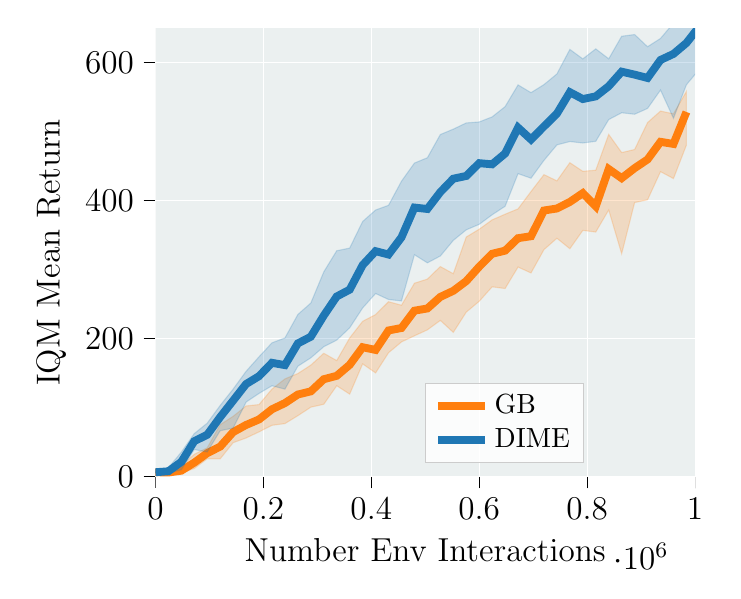
\begin{tikzpicture}

\definecolor{darkcyan1115178}{RGB}{1,115,178}
\definecolor{darkgray176}{RGB}{176,176,176}
\begin{axis}[
legend cell align={left},
legend cell align={left},
legend style={fill opacity=0.8, draw opacity=1, text opacity=1, draw=lightgray204, at={(0.5,0.03)},  anchor=south west},
tick align=outside,
tick pos=left,
x grid style={white},
xlabel={Number Env Interactions},
xmajorgrids,
%xmin=-37798.95, xmax=1045799.95,
xmin=-0.0, xmax=1000000.0,
xtick style={color=black},
y grid style={white},
ylabel={IQM Mean Return},
ymajorgrids,
ymin=-0.05, ymax=650,
ytick style={color=black},
axis background/.style={fill=plot_background},
label style={font=\large},
tick label style={font=\large},
x axis line style={draw=none},
y axis line style={draw=none},
]

\path [draw=C1, fill=C1, opacity=0.2]
(axis cs:1,6.99064241375)
--(axis cs:1,5.53621398333333)
--(axis cs:24000,4.28067333333333)
--(axis cs:48000,5.23071248333333)
--(axis cs:72000,11.5755848333333)
--(axis cs:96000,25.6408245)
--(axis cs:120000,25.5247493333333)
--(axis cs:144000,49.0188601666667)
--(axis cs:168000,55.8191148333333)
--(axis cs:192000,64.692345)
--(axis cs:216000,74.227769)
--(axis cs:240000,76.6928327708333)
--(axis cs:264000,88.1837003333333)
--(axis cs:288000,100.492174333333)
--(axis cs:312000,104.722368833333)
--(axis cs:336000,131.590808666667)
--(axis cs:360000,119.437102833333)
--(axis cs:384000,163.30507)
--(axis cs:408000,150.17637)
--(axis cs:432000,179.395848333333)
--(axis cs:456000,195.124558333333)
--(axis cs:480000,203.97069)
--(axis cs:504000,212.606669416667)
--(axis cs:528000,226.329041666667)
--(axis cs:552000,208.9856615)
--(axis cs:576000,238.283675)
--(axis cs:600000,254.046571666667)
--(axis cs:624000,275.016495)
--(axis cs:648000,272.557551666667)
--(axis cs:672000,303.745753333333)
--(axis cs:696000,295.1025)
--(axis cs:720000,328.943138333333)
--(axis cs:744000,345.448668333333)
--(axis cs:768000,330.267365)
--(axis cs:792000,356.852763333333)
--(axis cs:816000,354.461231666667)
--(axis cs:840000,386.447986666667)
--(axis cs:864000,322.969651)
--(axis cs:888000,397.20823375)
--(axis cs:912000,401.222951666667)
--(axis cs:936000,442.04175)
--(axis cs:960000,432.004991666667)
--(axis cs:984000,480.562826666667)
--(axis cs:984000,558.374366666667)
--(axis cs:984000,558.374366666667)
--(axis cs:960000,525.832104583333)
--(axis cs:936000,529.901533333333)
--(axis cs:912000,513.201521666667)
--(axis cs:888000,474.12895)
--(axis cs:864000,469.702438333333)
--(axis cs:840000,496.014085)
--(axis cs:816000,444.1255905)
--(axis cs:792000,442.521501666667)
--(axis cs:768000,455.044088333333)
--(axis cs:744000,428.69203)
--(axis cs:720000,437.708196666667)
--(axis cs:696000,413.18612)
--(axis cs:672000,388.057755)
--(axis cs:648000,380.312158333333)
--(axis cs:624000,372.099101666667)
--(axis cs:600000,358.568943333333)
--(axis cs:576000,347.241066666667)
--(axis cs:552000,294.06811)
--(axis cs:528000,304.411563333333)
--(axis cs:504000,286.250968333333)
--(axis cs:480000,280.257595)
--(axis cs:456000,248.37012)
--(axis cs:432000,253.453026666667)
--(axis cs:408000,234.7783)
--(axis cs:384000,224.984858333333)
--(axis cs:360000,200.886195)
--(axis cs:336000,168.093413333333)
--(axis cs:312000,178.664308291667)
--(axis cs:288000,161.485955)
--(axis cs:264000,149.313381666667)
--(axis cs:240000,141.529133333333)
--(axis cs:216000,126.745533333333)
--(axis cs:192000,104.314646666667)
--(axis cs:168000,102.2518335)
--(axis cs:144000,87.278177)
--(axis cs:120000,75.0973646666667)
--(axis cs:96000,41.588288)
--(axis cs:72000,32.1586941666667)
--(axis cs:48000,15.5923155745834)
--(axis cs:24000,8.6525861)
--(axis cs:1,6.99064241375)
--cycle;

\addplot [line width =\linewidthdime, C1, mark=*, mark size=0, mark options={solid}]
table {%
1 6.26247963333333
24000 5.7611181
48000 8.44131896666667
72000 20.1185598333333
96000 33.835471
120000 43.3480071666667
144000 64.3745236666667
168000 74.728139
192000 82.733837
216000 97.4774865
240000 106.443479166667
264000 118.875678333333
288000 123.44706
312000 141.0412925
336000 146.003979333333
360000 161.940301666667
384000 187.447373333333
408000 183.521465
432000 211.75379
456000 215.336466666667
480000 240.42844
504000 243.661463333333
528000 260.393455
552000 269.220865
576000 283.278935
600000 304.192728333333
624000 322.943031666667
648000 327.473726666667
672000 345.551548333333
696000 348.384485
720000 385.68403
744000 388.59085
768000 398.13177
792000 410.87024
816000 391.699205
840000 445.783146666667
864000 432.561828333333
888000 447.10136
912000 459.732565
936000 485.271595
960000 482.201818333333
984000 528.51851
};
\addlegendentry{GB}
%DIME
\path [draw=C0, fill=C0, opacity=0.2]
(axis cs:1,6.80215591666667)
--(axis cs:1,5.5925808)
--(axis cs:24000,4.88713573333333)
--(axis cs:48000,9.748871)
--(axis cs:72000,39.178405)
--(axis cs:96000,35.577766)
--(axis cs:120000,66.3638765)
--(axis cs:144000,70.247577)
--(axis cs:168000,107.848963333333)
--(axis cs:192000,120.425612666667)
--(axis cs:216000,131.606081666667)
--(axis cs:240000,126.6783995)
--(axis cs:264000,159.943133333333)
--(axis cs:288000,172.044628333333)
--(axis cs:312000,188.191985)
--(axis cs:336000,197.75034)
--(axis cs:360000,215.573404333333)
--(axis cs:384000,244.38039)
--(axis cs:408000,265.35188)
--(axis cs:432000,256.659486666667)
--(axis cs:456000,254.555695)
--(axis cs:480000,321.560075)
--(axis cs:504000,309.784411666667)
--(axis cs:528000,319.716291666667)
--(axis cs:552000,342.35053)
--(axis cs:576000,357.640175)
--(axis cs:600000,365.597093333333)
--(axis cs:624000,379.492581666667)
--(axis cs:648000,391.800683333333)
--(axis cs:672000,439.1368195)
--(axis cs:696000,432.521263333333)
--(axis cs:720000,458.362536666667)
--(axis cs:744000,480.79676)
--(axis cs:768000,485.700503333333)
--(axis cs:792000,483.583248791667)
--(axis cs:816000,485.992758916667)
--(axis cs:840000,517.541645)
--(axis cs:864000,527.38718)
--(axis cs:888000,525.263277708333)
--(axis cs:912000,533.699495)
--(axis cs:936000,560.338303333333)
--(axis cs:960000,519.453665)
--(axis cs:984000,568.020833333333)
--(axis cs:1008000,590.470613333333)
--(axis cs:1032000,581.025416666667)
--(axis cs:1056000,583.688265)
--(axis cs:1080000,607.528891666667)
--(axis cs:1104000,620.278735)
--(axis cs:1128000,613.026586666667)
--(axis cs:1152000,638.844431666667)
--(axis cs:1176000,637.409991666667)
--(axis cs:1200000,641.941126666667)
--(axis cs:1224000,658.54966)
--(axis cs:1248000,646.231282291667)
--(axis cs:1272000,671.152858333333)
--(axis cs:1296000,660.192991666667)
--(axis cs:1320000,670.868964125)
--(axis cs:1344000,672.098633333333)
--(axis cs:1368000,667.270646666667)
--(axis cs:1392000,679.406895)
--(axis cs:1416000,667.768826166667)
--(axis cs:1440000,699.8657)
--(axis cs:1464000,703.368514541667)
--(axis cs:1488000,691.688456666667)
--(axis cs:1512000,691.02705)
--(axis cs:1536000,724.245045)
--(axis cs:1560000,642.1076)
--(axis cs:1584000,677.059261666667)
--(axis cs:1608000,722.467075)
--(axis cs:1632000,724.970475)
--(axis cs:1656000,707.042333333333)
--(axis cs:1680000,723.18196)
--(axis cs:1704000,739.733563333333)
--(axis cs:1728000,732.09224)
--(axis cs:1752000,743.118561666667)
--(axis cs:1776000,697.080626666666)
--(axis cs:1800000,709.36812)
--(axis cs:1824000,650.052771666667)
--(axis cs:1848000,716.700755)
--(axis cs:1872000,731.219691458333)
--(axis cs:1896000,703.767975)
--(axis cs:1920000,748.827876666667)
--(axis cs:1944000,769.246855)
--(axis cs:1968000,752.894191666667)
--(axis cs:1992000,737.845081666667)
--(axis cs:2016000,756.439925)
--(axis cs:2040000,764.171413333333)
--(axis cs:2064000,740.270250333333)
--(axis cs:2088000,725.118516666667)
--(axis cs:2112000,743.246291625)
--(axis cs:2136000,734.83942)
--(axis cs:2160000,786.861907708333)
--(axis cs:2184000,738.508053333333)
--(axis cs:2208000,750.911366666667)
--(axis cs:2232000,786.895078333333)
--(axis cs:2256000,798.218891666667)
--(axis cs:2280000,758.322531666667)
--(axis cs:2304000,768.420973333333)
--(axis cs:2328000,798.43544325)
--(axis cs:2352000,735.766616666667)
--(axis cs:2376000,763.731855)
--(axis cs:2400000,788.471761666667)
--(axis cs:2424000,798.863623333333)
--(axis cs:2448000,797.623013333333)
--(axis cs:2472000,798.009976666667)
--(axis cs:2496000,799.156973333333)
--(axis cs:2520000,789.180108333333)
--(axis cs:2544000,793.308771666667)
--(axis cs:2568000,766.555433333333)
--(axis cs:2592000,775.906533333333)
--(axis cs:2616000,657.870696541667)
--(axis cs:2640000,802.967105)
--(axis cs:2664000,762.239025)
--(axis cs:2688000,758.85175)
--(axis cs:2712000,832.457286666667)
--(axis cs:2736000,798.855305)
--(axis cs:2760000,790.104215)
--(axis cs:2784000,817.637935)
--(axis cs:2808000,791.100776666667)
--(axis cs:2832000,821.486588458333)
--(axis cs:2856000,798.389748333333)
--(axis cs:2880000,756.81125)
--(axis cs:2904000,809.53344)
--(axis cs:2928000,784.753078333333)
--(axis cs:2952000,778.719458333333)
--(axis cs:2976000,756.92755)
--(axis cs:3000000,792.897486666667)
--(axis cs:3000000,837.456603333333)
--(axis cs:3000000,837.456603333333)
--(axis cs:2976000,848.466266666667)
--(axis cs:2952000,849.20779)
--(axis cs:2928000,842.088306666667)
--(axis cs:2904000,854.474571666667)
--(axis cs:2880000,849.331893333333)
--(axis cs:2856000,862.497737875)
--(axis cs:2832000,869.625008333333)
--(axis cs:2808000,863.616378333333)
--(axis cs:2784000,860.982908333333)
--(axis cs:2760000,837.8695)
--(axis cs:2736000,852.905353333333)
--(axis cs:2712000,861.954153333333)
--(axis cs:2688000,830.469433333333)
--(axis cs:2664000,868.63305)
--(axis cs:2640000,864.472063333333)
--(axis cs:2616000,836.439531666667)
--(axis cs:2592000,863.806)
--(axis cs:2568000,856.3503)
--(axis cs:2544000,854.31376)
--(axis cs:2520000,848.667223333333)
--(axis cs:2496000,852.5053125)
--(axis cs:2472000,847.29574)
--(axis cs:2448000,844.57391)
--(axis cs:2424000,851.800331666667)
--(axis cs:2400000,842.753173333333)
--(axis cs:2376000,851.53189)
--(axis cs:2352000,824.298165)
--(axis cs:2328000,854.002923333333)
--(axis cs:2304000,823.149833333333)
--(axis cs:2280000,842.485828333333)
--(axis cs:2256000,850.53472)
--(axis cs:2232000,834.622511666667)
--(axis cs:2208000,832.830438333333)
--(axis cs:2184000,829.092180333333)
--(axis cs:2160000,843.589423333333)
--(axis cs:2136000,835.928383333333)
--(axis cs:2112000,828.188466666667)
--(axis cs:2088000,834.338206875)
--(axis cs:2064000,847.99647)
--(axis cs:2040000,817.802191666667)
--(axis cs:2016000,831.623071666667)
--(axis cs:1992000,808.728928708333)
--(axis cs:1968000,824.828883333333)
--(axis cs:1944000,821.340061666667)
--(axis cs:1920000,826.504741666667)
--(axis cs:1896000,818.318428333333)
--(axis cs:1872000,831.390226666667)
--(axis cs:1848000,826.4945)
--(axis cs:1824000,819.049933333333)
--(axis cs:1800000,842.232765791667)
--(axis cs:1776000,826.921123333333)
--(axis cs:1752000,834.800166666667)
--(axis cs:1728000,837.246975)
--(axis cs:1704000,853.61177)
--(axis cs:1680000,810.376866666667)
--(axis cs:1656000,808.423789083334)
--(axis cs:1632000,821.8582)
--(axis cs:1608000,815.354633333333)
--(axis cs:1584000,808.92544)
--(axis cs:1560000,812.104926666667)
--(axis cs:1536000,809.656291666667)
--(axis cs:1512000,782.288026666667)
--(axis cs:1488000,778.782291583334)
--(axis cs:1464000,778.858313333333)
--(axis cs:1440000,821.10777)
--(axis cs:1416000,783.881986666667)
--(axis cs:1392000,750.93809425)
--(axis cs:1368000,760.521313333333)
--(axis cs:1344000,766.813391666667)
--(axis cs:1320000,745.988075)
--(axis cs:1296000,745.58748175)
--(axis cs:1272000,778.078543333333)
--(axis cs:1248000,739.945458333333)
--(axis cs:1224000,752.028946666667)
--(axis cs:1200000,754.479292041667)
--(axis cs:1176000,738.838393333333)
--(axis cs:1152000,730.995366666667)
--(axis cs:1128000,726.874316666667)
--(axis cs:1104000,706.711063333333)
--(axis cs:1080000,710.372623333333)
--(axis cs:1056000,691.064566666667)
--(axis cs:1032000,651.101731666667)
--(axis cs:1008000,694.859348333333)
--(axis cs:984000,679.811011666667)
--(axis cs:960000,657.437975)
--(axis cs:936000,635.207354333333)
--(axis cs:912000,623.17085)
--(axis cs:888000,640.82537)
--(axis cs:864000,638.372956666667)
--(axis cs:840000,605.636066666667)
--(axis cs:816000,620.0484)
--(axis cs:792000,605.530201666667)
--(axis cs:768000,619.288428333333)
--(axis cs:744000,583.706463333333)
--(axis cs:720000,568.233463333333)
--(axis cs:696000,556.574435)
--(axis cs:672000,567.827056666667)
--(axis cs:648000,536.300349125)
--(axis cs:624000,521.473436666667)
--(axis cs:600000,514.082965)
--(axis cs:576000,512.673896666667)
--(axis cs:552000,503.68212)
--(axis cs:528000,495.859381666667)
--(axis cs:504000,462.220926666667)
--(axis cs:480000,454.484963333333)
--(axis cs:456000,428.183936666667)
--(axis cs:432000,393.258111666667)
--(axis cs:408000,386.389815)
--(axis cs:384000,369.733846666667)
--(axis cs:360000,331.193968333333)
--(axis cs:336000,327.351346666667)
--(axis cs:312000,296.701976666667)
--(axis cs:288000,251.529673375)
--(axis cs:264000,234.932268333333)
--(axis cs:240000,200.893656666667)
--(axis cs:216000,193.835535)
--(axis cs:192000,173.552272666667)
--(axis cs:168000,152.488876666667)
--(axis cs:144000,126.71998265)
--(axis cs:120000,102.995841)
--(axis cs:96000,77.3036046666667)
--(axis cs:72000,62.1926506666667)
--(axis cs:48000,35.3083526666667)
--(axis cs:24000,12.7237687833333)
--(axis cs:1,6.80215591666667)
--cycle;

\addplot [line width=\linewidthdime, C0, mark=*, mark size=0, mark options={solid}]
table {%
1 6.17641296666667
24000 7.56386268333333
48000 21.194537
72000 51.2078703333333
96000 60.4982363333333
120000 86.1485583333333
144000 110.007961666667
168000 134.059945
192000 145.492449333333
216000 164.83243
240000 161.520515
264000 192.983695
288000 202.72266
312000 233.335831666667
336000 261.032931666667
360000 270.949796666667
384000 306.506178333333
408000 326.736271666667
432000 321.852778333333
456000 346.82201
480000 389.972858333333
504000 387.914375
528000 412.405621666667
552000 431.808476666667
576000 435.778751666667
600000 454.327343333333
624000 452.650095
648000 468.345228333333
672000 505.85564
696000 488.718146666667
720000 507.547415
744000 526.153453333333
768000 557.257588333333
792000 547.320155
816000 551.174743333333
840000 565.919836666667
864000 586.99087
888000 582.702056666667
912000 577.851651666667
936000 603.980191666667
960000 612.742416666667
984000 628.581438333333
1008000 652.547345
1032000 621.855605
1056000 653.459033333333
1080000 677.789983333333
1104000 677.092326666667
1128000 688.166816666667
1152000 696.043668333333
1176000 689.546143333333
1200000 707.716985
1224000 716.223413333333
1248000 695.373521666667
1272000 729.041578333333
1296000 711.299655
1320000 714.779295
1344000 720.93956
1368000 718.17746
1392000 720.170855
1416000 742.45139
1440000 767.977446666667
1464000 745.921991666667
1488000 741.981485
1512000 740.075188333334
1536000 776.043163333333
1560000 730.35288
1584000 745.76982
1608000 774.030058333333
1632000 786.423141666667
1656000 775.007413333333
1680000 767.966193333333
1704000 803.248776666667
1728000 795.057825
1752000 799.094
1776000 768.546685
1800000 785.936768333333
1824000 770.381045
1848000 778.163971666667
1872000 784.5074
1896000 775.084686666667
1920000 803.85685
1944000 802.98721
1968000 799.194371666667
1992000 777.64892
2016000 809.862228333333
2040000 802.882363333333
2064000 807.031923333333
2088000 792.892843333333
2112000 784.135861666667
2136000 799.080736666667
2160000 829.289918333333
2184000 812.669866666667
2208000 798.845955
2232000 810.922945
2256000 829.769393333333
2280000 808.989303333333
2304000 787.9255
2328000 834.55804
2352000 790.163291666667
2376000 809.844736666667
2400000 823.614375
2424000 829.909856666667
2448000 827.945956666667
2472000 830.88744
2496000 832.031106666667
2520000 821.356241666667
2544000 822.67606
2568000 821.050315
2592000 838.71875
2616000 819.876546666667
2640000 836.608795
2664000 842.476748333333
2688000 800.310716666667
2712000 848.692928333333
2736000 828.082728333333
2760000 814.163598333333
2784000 843.60977
2808000 840.753683333333
2832000 848.649233333333
2856000 840.45366
2880000 812.837433333333
2904000 839.813745
2928000 813.380873333333
2952000 813.313951666667
2976000 809.99765
3000000 818.333465
};
\addlegendentry{DIME}
\end{axis}

\end{tikzpicture}
}
       \subcaption[]{DIME and GB on Dog Run}
       \label{fig::appendix_dog_rund_dbs}
    \end{minipage}\hfill
    \begin{minipage}[b]{0.33\textwidth}
        \centering
       \resizebox{1\textwidth}{!}{% This file was created with tikzplotlib v0.10.1.
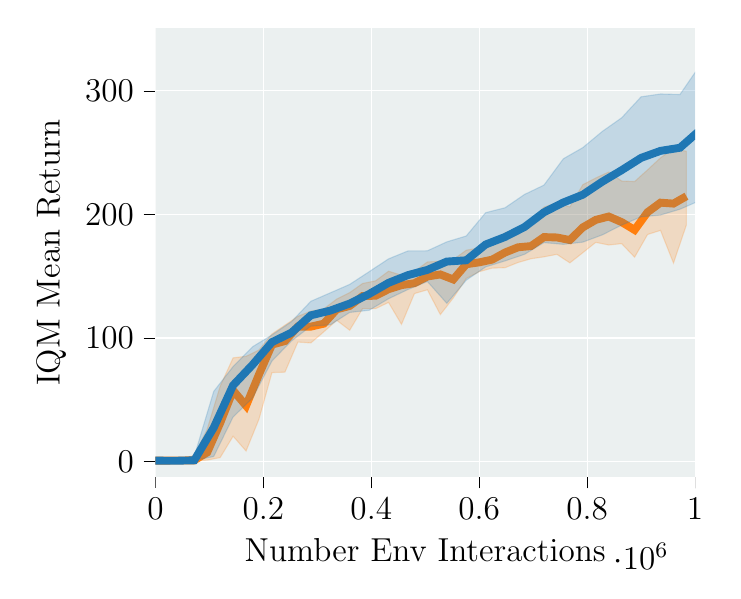
\begin{tikzpicture}

\definecolor{darkcyan1115178}{RGB}{1,115,178}
\definecolor{darkgray176}{RGB}{176,176,176}

\begin{axis}[
legend cell align={left},
legend cell align={left},
legend style={fill opacity=0.8, draw opacity=1, text opacity=1, draw=lightgray204, at={(0.5,0.03)},  anchor=south west},
tick align=outside,
tick pos=left,
x grid style={white},
xlabel={Number Env Interactions},
xmajorgrids,
xmin=-0.0, xmax=1000000.0,
xtick style={color=black},
y grid style={white},
ylabel={IQM Mean Return},
ymajorgrids,
ymin=-12.11232765065, ymax=350.65256879765,
ytick style={color=black},
axis background/.style={fill=plot_background},
label style={font=\large},
tick label style={font=\large},
x axis line style={draw=none},
y axis line style={draw=none},
]

\path [draw=C1, fill=C1, opacity=0.2]
(axis cs:1,0.913481333333333)
--(axis cs:1,0.6287236)
--(axis cs:24000,0.677781566666667)
--(axis cs:48000,0.738428966666667)
--(axis cs:72000,0.790174833333333)
--(axis cs:96000,1.1543524)
--(axis cs:120000,3.23502683000002)
--(axis cs:144000,20.5413528)
--(axis cs:168000,8.54387893333333)
--(axis cs:192000,34.4303118333333)
--(axis cs:216000,72.0098966666667)
--(axis cs:240000,72.3488675833333)
--(axis cs:264000,96.707165)
--(axis cs:288000,96.000784)
--(axis cs:312000,104.958421625)
--(axis cs:336000,114.297126)
--(axis cs:360000,106.284968)
--(axis cs:384000,123.7906925)
--(axis cs:408000,123.723489166667)
--(axis cs:432000,128.761211666667)
--(axis cs:456000,111.02938625)
--(axis cs:480000,135.956141666667)
--(axis cs:504000,138.98209)
--(axis cs:528000,118.929581333333)
--(axis cs:552000,132.387325)
--(axis cs:576000,148.148588333333)
--(axis cs:600000,153.61958)
--(axis cs:624000,156.55045)
--(axis cs:648000,156.870825)
--(axis cs:672000,161.074148333333)
--(axis cs:696000,164.107246666667)
--(axis cs:720000,165.654856541667)
--(axis cs:744000,167.669441666667)
--(axis cs:768000,160.786089)
--(axis cs:792000,168.99019)
--(axis cs:816000,177.369616666667)
--(axis cs:840000,175.239106666667)
--(axis cs:864000,176.361243333333)
--(axis cs:888000,165.394583333333)
--(axis cs:912000,183.752826666667)
--(axis cs:936000,187.066958333333)
--(axis cs:960000,160.625822716667)
--(axis cs:984000,191.555848333333)
--(axis cs:984000,251.074266666667)
--(axis cs:984000,251.074266666667)
--(axis cs:960000,253.124288333333)
--(axis cs:936000,245.776626666667)
--(axis cs:912000,236.034463333333)
--(axis cs:888000,226.598225)
--(axis cs:864000,227.013098708333)
--(axis cs:840000,234.283123333333)
--(axis cs:816000,229.472495)
--(axis cs:792000,224.034361666667)
--(axis cs:768000,206.047165)
--(axis cs:744000,209.549365)
--(axis cs:720000,205.859246666667)
--(axis cs:696000,194.984201666667)
--(axis cs:672000,188.552526666667)
--(axis cs:648000,185.157259583333)
--(axis cs:624000,177.684235)
--(axis cs:600000,172.894043333333)
--(axis cs:576000,171.0584)
--(axis cs:552000,163.391113333333)
--(axis cs:528000,162.135815)
--(axis cs:504000,161.517217666667)
--(axis cs:480000,153.846013166667)
--(axis cs:456000,150.815503333333)
--(axis cs:432000,154.043445)
--(axis cs:408000,146.23077)
--(axis cs:384000,144.130305)
--(axis cs:360000,136.713208333333)
--(axis cs:336000,131.509801666667)
--(axis cs:312000,123.557279541667)
--(axis cs:288000,121.774874166667)
--(axis cs:264000,117.476811666667)
--(axis cs:240000,110.350656666667)
--(axis cs:216000,103.274480333333)
--(axis cs:192000,90.3314516666667)
--(axis cs:168000,85.1717466666667)
--(axis cs:144000,83.9523868333333)
--(axis cs:120000,60.989724)
--(axis cs:96000,26.2789549666667)
--(axis cs:72000,5.35472753333333)
--(axis cs:48000,1.06001243333333)
--(axis cs:24000,0.923337466666667)
--(axis cs:1,0.913481333333333)
--cycle;

\addplot [line width=\linewidthdime, C1, mark=*, mark size=0, mark options={solid}]
table {%
1 0.7694417
24000 0.813880766666667
48000 0.903083466666667
72000 0.985341633333333
96000 7.39312896666667
120000 31.2267919666667
144000 57.5656945
168000 45.1603116666667
192000 70.5692
216000 94.6452396666667
240000 97.5139125
264000 109.186628333333
288000 109.1955065
312000 111.598211666667
336000 123.198625
360000 125.946167
384000 133.888621666667
408000 134.214293333333
432000 139.483735
456000 142.763216666667
480000 144.338755
504000 149.75221
528000 151.421726666667
552000 147.365006666667
576000 159.676698333333
600000 161.191491666667
624000 163.406718333333
648000 169.18849
672000 173.390193333333
696000 174.364796666667
720000 181.648728333333
744000 181.343818333333
768000 179.253028333333
792000 189.492575
816000 195.565436666667
840000 198.284515
864000 193.75859
888000 187.434418333333
912000 201.805691666667
936000 209.501925
960000 208.739933333333
984000 214.710998333333
};

%DIME
\path [draw=C0, fill=C0, opacity=0.2]
(axis cs:1,0.915501966666667)
--(axis cs:1,0.633556866666667)
--(axis cs:36000,0.5493304)
--(axis cs:72000,0.843873266666667)
--(axis cs:108000,4.13696455)
--(axis cs:144000,36.1211871666667)
--(axis cs:180000,51.4064937333333)
--(axis cs:216000,81.368514)
--(axis cs:252000,97.5408251666667)
--(axis cs:288000,109.583571666667)
--(axis cs:324000,110.618288333333)
--(axis cs:360000,120.684184666667)
--(axis cs:396000,122.417020833333)
--(axis cs:432000,131.747461666667)
--(axis cs:468000,139.23245)
--(axis cs:504000,145.708203333333)
--(axis cs:540000,128.071794166667)
--(axis cs:576000,146.743565)
--(axis cs:612000,157.523090333333)
--(axis cs:648000,162.386513333333)
--(axis cs:684000,167.712168333333)
--(axis cs:720000,177.17324)
--(axis cs:756000,175.778066666667)
--(axis cs:792000,177.557476666667)
--(axis cs:828000,183.413371666667)
--(axis cs:864000,191.343878333333)
--(axis cs:900000,198.058078333333)
--(axis cs:936000,199.495351666667)
--(axis cs:972000,204.18452)
--(axis cs:1008000,211.017165)
--(axis cs:1044000,210.395921666667)
--(axis cs:1080000,225.37889)
--(axis cs:1116000,225.57669)
--(axis cs:1152000,229.055506666667)
--(axis cs:1188000,244.717408333333)
--(axis cs:1224000,235.69925925)
--(axis cs:1260000,246.761671666667)
--(axis cs:1296000,263.70817)
--(axis cs:1332000,261.655338333333)
--(axis cs:1368000,274.904988333333)
--(axis cs:1404000,281.871765)
--(axis cs:1440000,284.6845)
--(axis cs:1476000,298.373705)
--(axis cs:1512000,314.234433333333)
--(axis cs:1548000,302.586606666667)
--(axis cs:1584000,306.158113166667)
--(axis cs:1620000,329.89694)
--(axis cs:1656000,327.346265)
--(axis cs:1692000,331.977616666667)
--(axis cs:1728000,335.598585)
--(axis cs:1764000,337.5854)
--(axis cs:1800000,350.510931458333)
--(axis cs:1836000,348.138216666667)
--(axis cs:1872000,325.377726666667)
--(axis cs:1908000,375.064071666667)
--(axis cs:1944000,364.504996666667)
--(axis cs:1980000,362.576775)
--(axis cs:2016000,359.905746666667)
--(axis cs:2052000,401.565295)
--(axis cs:2088000,380.944233333333)
--(axis cs:2124000,408.07439)
--(axis cs:2160000,406.816443333333)
--(axis cs:2196000,402.540623333333)
--(axis cs:2232000,419.828846666667)
--(axis cs:2268000,419.407693333333)
--(axis cs:2304000,391.893025)
--(axis cs:2340000,426.646173333333)
--(axis cs:2376000,430.59703)
--(axis cs:2412000,440.944021375)
--(axis cs:2448000,444.535958333333)
--(axis cs:2484000,447.59097)
--(axis cs:2520000,458.220718125)
--(axis cs:2556000,454.987311666667)
--(axis cs:2592000,444.593778333333)
--(axis cs:2628000,452.355353333333)
--(axis cs:2664000,472.315071583333)
--(axis cs:2700000,468.552297125)
--(axis cs:2736000,425.893185)
--(axis cs:2772000,461.17882)
--(axis cs:2808000,438.974565)
--(axis cs:2844000,408.566183333333)
--(axis cs:2880000,440.493023333333)
--(axis cs:2916000,474.594651666667)
--(axis cs:2952000,473.13282)
--(axis cs:2988000,468.31128725)
--(axis cs:2988000,572.54452975)
--(axis cs:2988000,572.54452975)
--(axis cs:2952000,607.047773333333)
--(axis cs:2916000,581.955683333333)
--(axis cs:2880000,562.69891)
--(axis cs:2844000,570.399441666667)
--(axis cs:2808000,561.294171666667)
--(axis cs:2772000,575.424046666667)
--(axis cs:2736000,577.564579375)
--(axis cs:2700000,570.731558333333)
--(axis cs:2664000,556.645568333333)
--(axis cs:2628000,528.610636666667)
--(axis cs:2592000,572.906766666667)
--(axis cs:2556000,556.792031666667)
--(axis cs:2520000,565.548321666667)
--(axis cs:2484000,564.076643333333)
--(axis cs:2448000,554.428711666667)
--(axis cs:2412000,511.028458333333)
--(axis cs:2376000,539.327213333333)
--(axis cs:2340000,521.274179458333)
--(axis cs:2304000,507.011033333333)
--(axis cs:2268000,533.545403333333)
--(axis cs:2232000,530.436551666667)
--(axis cs:2196000,514.156165)
--(axis cs:2160000,548.6599)
--(axis cs:2124000,526.241701666667)
--(axis cs:2088000,488.449933333333)
--(axis cs:2052000,521.397975)
--(axis cs:2016000,489.724498333333)
--(axis cs:1980000,511.56874)
--(axis cs:1944000,469.79517)
--(axis cs:1908000,487.4035)
--(axis cs:1872000,452.261116666667)
--(axis cs:1836000,448.443288333333)
--(axis cs:1800000,470.013476541667)
--(axis cs:1764000,441.067136666667)
--(axis cs:1728000,425.983283333333)
--(axis cs:1692000,459.900376666667)
--(axis cs:1656000,420.555463333333)
--(axis cs:1620000,452.412428333333)
--(axis cs:1584000,426.080911666667)
--(axis cs:1548000,405.744391916667)
--(axis cs:1512000,422.468795)
--(axis cs:1476000,392.121763333333)
--(axis cs:1440000,398.927006666667)
--(axis cs:1404000,396.300881666667)
--(axis cs:1368000,391.708926666667)
--(axis cs:1332000,379.3367)
--(axis cs:1296000,374.028266666667)
--(axis cs:1260000,354.826833333333)
--(axis cs:1224000,325.77437)
--(axis cs:1188000,356.78896)
--(axis cs:1152000,352.524811666667)
--(axis cs:1116000,343.294016666667)
--(axis cs:1080000,331.116815)
--(axis cs:1044000,287.783165)
--(axis cs:1008000,319.938826666667)
--(axis cs:972000,297.00894)
--(axis cs:936000,297.43841)
--(axis cs:900000,295.160138333333)
--(axis cs:864000,278.186283333333)
--(axis cs:828000,267.117865)
--(axis cs:792000,254.04739775)
--(axis cs:756000,245.040613333333)
--(axis cs:720000,223.696456875)
--(axis cs:684000,216.1656)
--(axis cs:648000,205.401713333333)
--(axis cs:612000,201.404601666667)
--(axis cs:576000,182.55503)
--(axis cs:540000,177.786793333333)
--(axis cs:504000,170.561265208333)
--(axis cs:468000,170.450261666667)
--(axis cs:432000,164.02998)
--(axis cs:396000,153.633991666667)
--(axis cs:360000,143.37209)
--(axis cs:324000,136.525775833333)
--(axis cs:288000,129.716861683333)
--(axis cs:252000,113.1404125)
--(axis cs:216000,102.49002)
--(axis cs:180000,92.9197603333333)
--(axis cs:144000,76.8890066666667)
--(axis cs:108000,56.7536433333333)
--(axis cs:72000,4.25857906666667)
--(axis cs:36000,0.728938933333333)
--(axis cs:1,0.915501966666667)
--cycle;

\addplot [line width=\linewidthdime, C0, mark=*, mark size=0, mark options={solid}]
table {%
1 0.770562166666667
36000 0.658370533333333
72000 1.02744053333333
108000 27.4132359166667
144000 61.7389005
180000 78.3388245
216000 96.6475441666667
252000 104.292225666667
288000 118.336289333333
324000 122.156900833333
360000 127.865645666667
396000 135.589655833333
432000 144.61231
468000 150.876916666667
504000 155.106371666667
540000 161.848961666667
576000 162.873085
612000 175.66877
648000 181.774033333333
684000 189.795443333333
720000 201.694543333333
756000 209.679653333333
792000 215.950858333333
828000 226.452128333333
864000 235.790758333333
900000 245.745095
936000 251.419853333333
972000 253.923228333333
1008000 267.745066666667
1044000 253.029908333333
1080000 281.1757
1116000 290.478148333333
1152000 295.386573333333
1188000 307.510898333333
1224000 279.324226666667
1260000 298.499671666667
1296000 320.530285
1332000 314.688511666667
1368000 333.564955
1404000 344.035705
1440000 351.026203333333
1476000 334.48205
1512000 371.517083333333
1548000 359.107073333333
1584000 362.49581
1620000 383.735268333333
1656000 371.120853333333
1692000 392.875408333333
1728000 375.706403333333
1764000 385.148411666667
1800000 411.377563333333
1836000 393.022041666667
1872000 381.083618333333
1908000 428.514751666667
1944000 407.976545
1980000 440.522148333333
2016000 425.096363333333
2052000 460.246375
2088000 439.221346666667
2124000 470.482476666667
2160000 479.806223333333
2196000 467.028006666667
2232000 471.833656666667
2268000 492.305195
2304000 444.283438333333
2340000 467.734686666667
2376000 478.305563333333
2412000 479.659883333333
2448000 502.891963333333
2484000 512.254108333333
2520000 504.927955
2556000 509.89631
2592000 517.465808333333
2628000 505.843831666667
2664000 503.219516666667
2700000 525.334166666667
2736000 498.718568333333
2772000 515.273173333333
2808000 507.004858333333
2844000 490.845221666667
2880000 488.33129
2916000 530.288801666667
2952000 544.121438333333
2988000 506.351106666667
};

\end{axis}

\end{tikzpicture}
}
       \subcaption[]{DIME and GB on Humanoid Run}
       \label{fig::appendix_hum_rund_dbs}
    \end{minipage}\hfill
    \begin{minipage}[b]{0.33\textwidth}
        \centering
       \resizebox{1\textwidth}{!}{\definecolor{crimson2143940}{RGB}{214,39,40}
\definecolor{darkgray176}{RGB}{176,176,176}
\definecolor{darkorange25512714}{RGB}{255,127,14}
\definecolor{forestgreen4416044}{RGB}{44,160,44}
\definecolor{mediumpurple148103189}{RGB}{148,103,189}
\definecolor{steelblue31119180}{RGB}{31,119,180}

% This file was created with tikzplotlib v0.10.1.
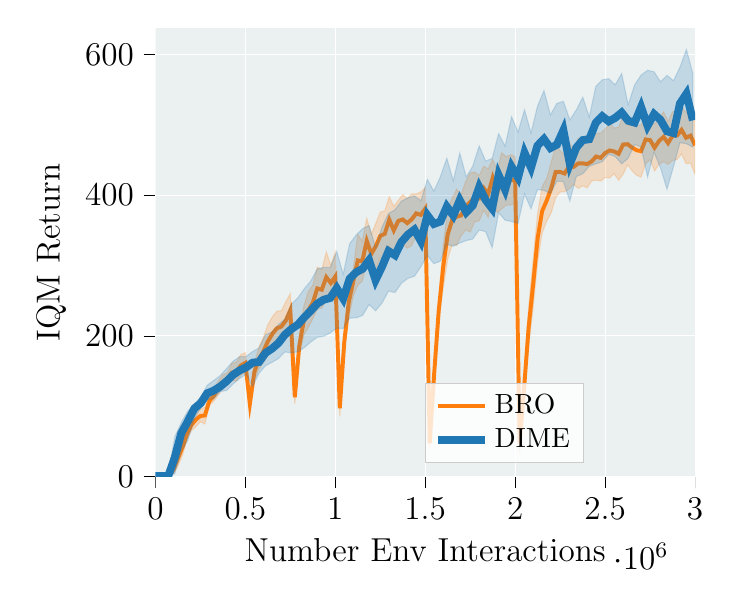
\begin{tikzpicture}

\definecolor{darkcyan1115178}{RGB}{1,115,178}
\definecolor{darkgray176}{RGB}{176,176,176}

\begin{axis}[
legend cell align={left},
legend cell align={left},
legend style={fill opacity=0.8, draw opacity=1, text opacity=1, draw=lightgray204, at={(0.5,0.03)},  anchor=south west},
tick align=outside,
tick pos=left,
x grid style={white},
xlabel={Number Env Interactions},
xmajorgrids,
%xmin=-149398.95, xmax=3000000.00,
xmin=0.0, xmax=3000000.00,
xtick style={color=black},
y grid style={white},
ylabel={IQM Return},
ymajorgrids,
%ymin=-37.9926843766667, ymax=923.09120151,
ymin=0.0, ymax=637.37269548,
ytick style={color=black},
axis background/.style={fill=plot_background},
label style={font=\large},
tick label style={font=\large},
x axis line style={draw=none},
y axis line style={draw=none},
]
% BRO

\path [draw=C1, fill=C1, opacity=0.2]
(axis cs:25000,1.06436189695316)
--(axis cs:25000,0.800044970854062)
--(axis cs:50000,0.902213431331389)
--(axis cs:75000,0.998039782938274)
--(axis cs:100000,3.73818093255901)
--(axis cs:125000,14.8008643633554)
--(axis cs:150000,29.8200848291147)
--(axis cs:175000,52.536500676349)
--(axis cs:200000,65.4528765036023)
--(axis cs:225000,70.6547353460924)
--(axis cs:250000,77.9210714654044)
--(axis cs:275000,74.6925274736162)
--(axis cs:300000,101.688198709863)
--(axis cs:325000,107.281306117989)
--(axis cs:350000,115.959467727732)
--(axis cs:375000,124.884927566366)
--(axis cs:400000,129.951946684364)
--(axis cs:425000,136.152626975576)
--(axis cs:450000,136.111337375472)
--(axis cs:475000,143.874927358078)
--(axis cs:500000,148.567262987423)
--(axis cs:525000,94.5117370449074)
--(axis cs:550000,137.525904720989)
--(axis cs:575000,152.664260638624)
--(axis cs:600000,161.929930494808)
--(axis cs:625000,171.58650975503)
--(axis cs:650000,181.142500891986)
--(axis cs:675000,186.720413352857)
--(axis cs:700000,191.754617425019)
--(axis cs:725000,196.874121030149)
--(axis cs:750000,212.645896156586)
--(axis cs:775000,103.542898066904)
--(axis cs:800000,171.614039449506)
--(axis cs:825000,201.242993560958)
--(axis cs:850000,211.747982944836)
--(axis cs:875000,224.177397591092)
--(axis cs:900000,237.999427608921)
--(axis cs:925000,239.436421657841)
--(axis cs:950000,250.973926888014)
--(axis cs:975000,250.707118365674)
--(axis cs:1000000,255.7721777332)
--(axis cs:1025000,85.7462506497815)
--(axis cs:1050000,177.039576732904)
--(axis cs:1075000,226.850952562221)
--(axis cs:1100000,256.461162193783)
--(axis cs:1125000,272.077354487363)
--(axis cs:1150000,277.88091019911)
--(axis cs:1175000,302.440032278388)
--(axis cs:1200000,286.286261722487)
--(axis cs:1225000,295.097707667798)
--(axis cs:1250000,310.062918562881)
--(axis cs:1275000,310.671213558559)
--(axis cs:1300000,328.891560548388)
--(axis cs:1325000,315.261131031065)
--(axis cs:1350000,333.264653443051)
--(axis cs:1375000,330.201890430345)
--(axis cs:1400000,324.50649705123)
--(axis cs:1425000,328.421995352062)
--(axis cs:1450000,343.634546505786)
--(axis cs:1475000,339.296630224071)
--(axis cs:1500000,348.984178695933)
--(axis cs:1525000,39.355588180581)
--(axis cs:1550000,132.834147960603)
--(axis cs:1575000,220.885853788656)
--(axis cs:1600000,268.221180119728)
--(axis cs:1625000,309.413007126434)
--(axis cs:1650000,330.020327352981)
--(axis cs:1675000,328.810183948437)
--(axis cs:1700000,342.485717291448)
--(axis cs:1725000,350.558346157369)
--(axis cs:1750000,347.543642435759)
--(axis cs:1775000,362.036408929491)
--(axis cs:1800000,363.429130292646)
--(axis cs:1825000,378.249045471367)
--(axis cs:1850000,368.466818930279)
--(axis cs:1875000,395.92381129835)
--(axis cs:1900000,375.255770601223)
--(axis cs:1925000,380.466843316452)
--(axis cs:1950000,385.742622584488)
--(axis cs:1975000,385.833705784746)
--(axis cs:2000000,388.274637595042)
--(axis cs:2025000,33.5649937116025)
--(axis cs:2050000,109.201720408668)
--(axis cs:2075000,186.449238204214)
--(axis cs:2100000,240.623289727134)
--(axis cs:2125000,305.664385445925)
--(axis cs:2150000,346.718313109583)
--(axis cs:2175000,362.847691076416)
--(axis cs:2200000,374.670521199756)
--(axis cs:2225000,396.743614451708)
--(axis cs:2250000,404.508816918751)
--(axis cs:2275000,404.815724919529)
--(axis cs:2300000,408.67455149964)
--(axis cs:2325000,415.555724534537)
--(axis cs:2350000,409.515642698911)
--(axis cs:2375000,413.456404646793)
--(axis cs:2400000,410.346599855339)
--(axis cs:2425000,420.13357683042)
--(axis cs:2450000,421.419850504902)
--(axis cs:2475000,420.083915472082)
--(axis cs:2500000,425.007581951612)
--(axis cs:2525000,424.579049671924)
--(axis cs:2550000,430.75366994294)
--(axis cs:2575000,421.216107533729)
--(axis cs:2600000,429.76793736549)
--(axis cs:2625000,443.105374475612)
--(axis cs:2650000,434.722857001578)
--(axis cs:2675000,428.275377228427)
--(axis cs:2700000,425.81611641096)
--(axis cs:2725000,444.64365130971)
--(axis cs:2750000,450.413269764893)
--(axis cs:2775000,434.345878022504)
--(axis cs:2800000,443.91301212502)
--(axis cs:2825000,447.49939896642)
--(axis cs:2850000,443.697419471331)
--(axis cs:2875000,449.354555033438)
--(axis cs:2900000,450.8026245623)
--(axis cs:2925000,458.680244532348)
--(axis cs:2950000,444.916782676853)
--(axis cs:2975000,445.634457360389)
--(axis cs:3000000,429.880019721412)
--(axis cs:3000000,513.9873176354)
--(axis cs:3000000,513.9873176354)
--(axis cs:2975000,523.797044053664)
--(axis cs:2950000,517.810496299027)
--(axis cs:2925000,525.954271943104)
--(axis cs:2900000,518.551529862146)
--(axis cs:2875000,518.920986906444)
--(axis cs:2850000,505.088500000573)
--(axis cs:2825000,518.566273395142)
--(axis cs:2800000,509.237923377759)
--(axis cs:2775000,501.25737445807)
--(axis cs:2750000,505.642689921167)
--(axis cs:2725000,513.254245513279)
--(axis cs:2700000,499.87053006485)
--(axis cs:2675000,499.068414301387)
--(axis cs:2650000,499.244308228539)
--(axis cs:2625000,500.18961766769)
--(axis cs:2600000,512.531552452399)
--(axis cs:2575000,496.697448428239)
--(axis cs:2550000,495.403692454602)
--(axis cs:2525000,502.740522809381)
--(axis cs:2500000,493.846745259791)
--(axis cs:2475000,488.320572719053)
--(axis cs:2450000,487.649215256229)
--(axis cs:2425000,478.718572892562)
--(axis cs:2400000,477.202876793975)
--(axis cs:2375000,476.451092629711)
--(axis cs:2350000,481.167057793168)
--(axis cs:2325000,464.822365433921)
--(axis cs:2300000,475.130801215997)
--(axis cs:2275000,457.275923790936)
--(axis cs:2250000,463.437629737087)
--(axis cs:2225000,469.693586932296)
--(axis cs:2200000,446.464641236289)
--(axis cs:2175000,423.741760297603)
--(axis cs:2150000,412.259115726332)
--(axis cs:2125000,374.619709027751)
--(axis cs:2100000,308.103900280336)
--(axis cs:2075000,240.504027337852)
--(axis cs:2050000,147.589375617486)
--(axis cs:2025000,60.8440314157716)
--(axis cs:2000000,454.6140241901)
--(axis cs:1975000,457.782889455546)
--(axis cs:1950000,454.490153888389)
--(axis cs:1925000,460.646195395525)
--(axis cs:1900000,435.379018582715)
--(axis cs:1875000,451.043381396628)
--(axis cs:1850000,437.594051329755)
--(axis cs:1825000,441.161889244782)
--(axis cs:1800000,428.1258205615)
--(axis cs:1775000,433.047391857064)
--(axis cs:1750000,431.680207172047)
--(axis cs:1725000,419.626783286342)
--(axis cs:1700000,401.334051733191)
--(axis cs:1675000,408.532521204368)
--(axis cs:1650000,395.947013655237)
--(axis cs:1625000,381.209360225348)
--(axis cs:1600000,328.600370144145)
--(axis cs:1575000,252.603144263693)
--(axis cs:1550000,162.227344584328)
--(axis cs:1525000,55.3468262239898)
--(axis cs:1500000,410.792177821071)
--(axis cs:1475000,404.502694934256)
--(axis cs:1450000,401.813256783996)
--(axis cs:1425000,401.708044362734)
--(axis cs:1400000,395.125789323197)
--(axis cs:1375000,400.825515156559)
--(axis cs:1350000,392.647754460344)
--(axis cs:1325000,384.152222205941)
--(axis cs:1300000,397.852872002416)
--(axis cs:1275000,377.552362447173)
--(axis cs:1250000,376.011972574837)
--(axis cs:1225000,359.739845675417)
--(axis cs:1200000,344.509178975306)
--(axis cs:1175000,367.154285866658)
--(axis cs:1150000,334.799456193374)
--(axis cs:1125000,344.307719911651)
--(axis cs:1100000,296.227318401859)
--(axis cs:1075000,266.643166383648)
--(axis cs:1050000,204.584202057326)
--(axis cs:1025000,108.689802307726)
--(axis cs:1000000,318.852715650748)
--(axis cs:975000,300.456149902442)
--(axis cs:950000,319.33259299771)
--(axis cs:925000,294.26813015175)
--(axis cs:900000,297.854696283069)
--(axis cs:875000,272.025279001709)
--(axis cs:850000,263.353273415112)
--(axis cs:825000,242.24173443444)
--(axis cs:800000,200.105312087152)
--(axis cs:775000,122.615578156031)
--(axis cs:750000,259.997946552285)
--(axis cs:725000,248.381254652691)
--(axis cs:700000,235.75254015339)
--(axis cs:675000,235.151123818793)
--(axis cs:650000,227.018726493552)
--(axis cs:625000,215.921378426131)
--(axis cs:600000,197.741080859391)
--(axis cs:575000,183.93247982137)
--(axis cs:550000,160.853477460561)
--(axis cs:525000,112.900779876465)
--(axis cs:500000,176.061616899139)
--(axis cs:475000,173.423721376022)
--(axis cs:450000,162.489487033554)
--(axis cs:425000,161.259046819264)
--(axis cs:400000,147.344859501089)
--(axis cs:375000,144.659394938876)
--(axis cs:350000,136.178883223972)
--(axis cs:325000,123.99330842961)
--(axis cs:300000,113.533585440671)
--(axis cs:275000,98.6956458394326)
--(axis cs:250000,95.6263797325166)
--(axis cs:225000,90.8477919575314)
--(axis cs:200000,80.6211055761968)
--(axis cs:175000,68.9779022961458)
--(axis cs:150000,52.6168055078161)
--(axis cs:125000,37.2068416693329)
--(axis cs:100000,17.4181970842278)
--(axis cs:75000,1.58356256613591)
--(axis cs:50000,1.25625000054544)
--(axis cs:25000,1.06436189695316)
--cycle;

\addplot [line width=\linewidthother, C1, mark=*, mark size=0, mark options={solid}]
table {%
25000 0.930442202091521
50000 1.07651185871321
75000 1.25993092696276
100000 9.83030688967838
125000 25.6411418517771
150000 41.1075536267594
175000 60.3883914444651
200000 73.172436582942
225000 80.957633586035
250000 86.0890838978233
275000 86.8321797068196
300000 107.266605289419
325000 114.972760323541
350000 125.514097446969
375000 134.324845411907
400000 138.233436327078
425000 147.660369336518
450000 148.782457916996
475000 157.754543249098
500000 161.480475192749
525000 103.279940413761
550000 148.67370118324
575000 166.636231776283
600000 177.730272953984
625000 192.167083171252
650000 202.772177321453
675000 210.734125891453
700000 213.205316409278
725000 221.706877576317
750000 236.467345033334
775000 112.87857606821
800000 186.130552121398
825000 221.723558177307
850000 236.209271737391
875000 247.087024794249
900000 267.471165250301
925000 265.658479214331
950000 283.439134541734
975000 275.133379987545
1000000 284.437051242526
1025000 97.0758468913518
1050000 191.453500474107
1075000 247.925237545804
1100000 277.620995193895
1125000 307.245282942146
1150000 305.919661019263
1175000 335.107741080569
1200000 316.435912664741
1225000 327.456512993191
1250000 342.107967490487
1275000 345.094845414729
1300000 365.251258681473
1325000 349.916712906547
1350000 363.318109792082
1375000 365.501578733968
1400000 360.257954947648
1425000 365.685379120745
1450000 374.145117409919
1475000 372.055178318366
1500000 380.772709979235
1525000 47.1556118690389
1550000 147.391608013536
1575000 235.725959616489
1600000 298.100854291553
1625000 344.459721335641
1650000 364.712840460148
1675000 369.42338730188
1700000 371.318808438126
1725000 383.874329652056
1750000 390.530684839555
1775000 396.82664916639
1800000 395.408529222678
1825000 409.974986250516
1850000 401.761351799987
1875000 424.544214100914
1900000 403.427991613482
1925000 421.452086824094
1950000 420.168662455335
1975000 421.239853255038
2000000 421.557400426789
2025000 46.8497645215133
2050000 127.574579390775
2075000 212.337561217824
2100000 273.695465882477
2125000 339.060702704761
2150000 377.404140539549
2175000 392.147298960786
2200000 409.585928423078
2225000 432.930123927388
2250000 433.06954152684
2275000 430.817714378362
2300000 441.242333227845
2325000 440.26544618574
2350000 445.109444370395
2375000 445.310468474792
2400000 444.23401205299
2425000 447.974403762188
2450000 455.009836622286
2475000 453.065691276495
2500000 459.824261297809
2525000 463.614242587133
2550000 462.153633274131
2575000 458.885605928128
2600000 472.045677739907
2625000 472.465960920779
2650000 467.617349708702
2675000 463.919322456368
2700000 462.572175194156
2725000 479.223260869987
2750000 478.300271910278
2775000 467.550224472069
2800000 477.243281641589
2825000 482.77498600685
2850000 474.021199131709
2875000 484.511658494648
2900000 484.88515836079
2925000 492.783683602026
2950000 481.675038930042
2975000 484.59483344476
3000000 470.838626791646
};
\addlegendentry{BRO}
% DIME
\path [draw=C0, fill=C0, opacity=0.2]
(axis cs:1,0.915501966666667)
--(axis cs:1,0.633556866666667)
--(axis cs:36000,0.5493304)
--(axis cs:72000,0.843873266666667)
--(axis cs:108000,4.13696455)
--(axis cs:144000,36.1211871666667)
--(axis cs:180000,51.4064937333333)
--(axis cs:216000,81.368514)
--(axis cs:252000,97.5408251666667)
--(axis cs:288000,109.583571666667)
--(axis cs:324000,110.618288333333)
--(axis cs:360000,120.684184666667)
--(axis cs:396000,122.417020833333)
--(axis cs:432000,131.747461666667)
--(axis cs:468000,139.23245)
--(axis cs:504000,145.708203333333)
--(axis cs:540000,128.071794166667)
--(axis cs:576000,146.743565)
--(axis cs:612000,157.523090333333)
--(axis cs:648000,162.386513333333)
--(axis cs:684000,167.712168333333)
--(axis cs:720000,177.17324)
--(axis cs:756000,175.778066666667)
--(axis cs:792000,177.557476666667)
--(axis cs:828000,183.413371666667)
--(axis cs:864000,191.343878333333)
--(axis cs:900000,198.058078333333)
--(axis cs:936000,199.495351666667)
--(axis cs:972000,204.18452)
--(axis cs:1008000,211.017165)
--(axis cs:1044000,210.395921666667)
--(axis cs:1080000,225.37889)
--(axis cs:1116000,225.57669)
--(axis cs:1152000,229.055506666667)
--(axis cs:1188000,244.717408333333)
--(axis cs:1224000,235.69925925)
--(axis cs:1260000,246.761671666667)
--(axis cs:1296000,263.70817)
--(axis cs:1332000,261.655338333333)
--(axis cs:1368000,274.904988333333)
--(axis cs:1404000,281.871765)
--(axis cs:1440000,284.6845)
--(axis cs:1476000,298.373705)
--(axis cs:1512000,314.234433333333)
--(axis cs:1548000,302.586606666667)
--(axis cs:1584000,306.158113166667)
--(axis cs:1620000,329.89694)
--(axis cs:1656000,327.346265)
--(axis cs:1692000,331.977616666667)
--(axis cs:1728000,335.598585)
--(axis cs:1764000,337.5854)
--(axis cs:1800000,350.510931458333)
--(axis cs:1836000,348.138216666667)
--(axis cs:1872000,325.377726666667)
--(axis cs:1908000,375.064071666667)
--(axis cs:1944000,364.504996666667)
--(axis cs:1980000,362.576775)
--(axis cs:2016000,359.905746666667)
--(axis cs:2052000,401.565295)
--(axis cs:2088000,380.944233333333)
--(axis cs:2124000,408.07439)
--(axis cs:2160000,406.816443333333)
--(axis cs:2196000,402.540623333333)
--(axis cs:2232000,419.828846666667)
--(axis cs:2268000,419.407693333333)
--(axis cs:2304000,391.893025)
--(axis cs:2340000,426.646173333333)
--(axis cs:2376000,430.59703)
--(axis cs:2412000,440.944021375)
--(axis cs:2448000,444.535958333333)
--(axis cs:2484000,447.59097)
--(axis cs:2520000,458.220718125)
--(axis cs:2556000,454.987311666667)
--(axis cs:2592000,444.593778333333)
--(axis cs:2628000,452.355353333333)
--(axis cs:2664000,472.315071583333)
--(axis cs:2700000,468.552297125)
--(axis cs:2736000,425.893185)
--(axis cs:2772000,461.17882)
--(axis cs:2808000,438.974565)
--(axis cs:2844000,408.566183333333)
--(axis cs:2880000,440.493023333333)
--(axis cs:2916000,474.594651666667)
--(axis cs:2952000,473.13282)
--(axis cs:2988000,468.31128725)
--(axis cs:2988000,572.54452975)
--(axis cs:2988000,572.54452975)
--(axis cs:2952000,607.047773333333)
--(axis cs:2916000,581.955683333333)
--(axis cs:2880000,562.69891)
--(axis cs:2844000,570.399441666667)
--(axis cs:2808000,561.294171666667)
--(axis cs:2772000,575.424046666667)
--(axis cs:2736000,577.564579375)
--(axis cs:2700000,570.731558333333)
--(axis cs:2664000,556.645568333333)
--(axis cs:2628000,528.610636666667)
--(axis cs:2592000,572.906766666667)
--(axis cs:2556000,556.792031666667)
--(axis cs:2520000,565.548321666667)
--(axis cs:2484000,564.076643333333)
--(axis cs:2448000,554.428711666667)
--(axis cs:2412000,511.028458333333)
--(axis cs:2376000,539.327213333333)
--(axis cs:2340000,521.274179458333)
--(axis cs:2304000,507.011033333333)
--(axis cs:2268000,533.545403333333)
--(axis cs:2232000,530.436551666667)
--(axis cs:2196000,514.156165)
--(axis cs:2160000,548.6599)
--(axis cs:2124000,526.241701666667)
--(axis cs:2088000,488.449933333333)
--(axis cs:2052000,521.397975)
--(axis cs:2016000,489.724498333333)
--(axis cs:1980000,511.56874)
--(axis cs:1944000,469.79517)
--(axis cs:1908000,487.4035)
--(axis cs:1872000,452.261116666667)
--(axis cs:1836000,448.443288333333)
--(axis cs:1800000,470.013476541667)
--(axis cs:1764000,441.067136666667)
--(axis cs:1728000,425.983283333333)
--(axis cs:1692000,459.900376666667)
--(axis cs:1656000,420.555463333333)
--(axis cs:1620000,452.412428333333)
--(axis cs:1584000,426.080911666667)
--(axis cs:1548000,405.744391916667)
--(axis cs:1512000,422.468795)
--(axis cs:1476000,392.121763333333)
--(axis cs:1440000,398.927006666667)
--(axis cs:1404000,396.300881666667)
--(axis cs:1368000,391.708926666667)
--(axis cs:1332000,379.3367)
--(axis cs:1296000,374.028266666667)
--(axis cs:1260000,354.826833333333)
--(axis cs:1224000,325.77437)
--(axis cs:1188000,356.78896)
--(axis cs:1152000,352.524811666667)
--(axis cs:1116000,343.294016666667)
--(axis cs:1080000,331.116815)
--(axis cs:1044000,287.783165)
--(axis cs:1008000,319.938826666667)
--(axis cs:972000,297.00894)
--(axis cs:936000,297.43841)
--(axis cs:900000,295.160138333333)
--(axis cs:864000,278.186283333333)
--(axis cs:828000,267.117865)
--(axis cs:792000,254.04739775)
--(axis cs:756000,245.040613333333)
--(axis cs:720000,223.696456875)
--(axis cs:684000,216.1656)
--(axis cs:648000,205.401713333333)
--(axis cs:612000,201.404601666667)
--(axis cs:576000,182.55503)
--(axis cs:540000,177.786793333333)
--(axis cs:504000,170.561265208333)
--(axis cs:468000,170.450261666667)
--(axis cs:432000,164.02998)
--(axis cs:396000,153.633991666667)
--(axis cs:360000,143.37209)
--(axis cs:324000,136.525775833333)
--(axis cs:288000,129.716861683333)
--(axis cs:252000,113.1404125)
--(axis cs:216000,102.49002)
--(axis cs:180000,92.9197603333333)
--(axis cs:144000,76.8890066666667)
--(axis cs:108000,56.7536433333333)
--(axis cs:72000,4.25857906666667)
--(axis cs:36000,0.728938933333333)
--(axis cs:1,0.915501966666667)
--cycle;

\addplot [line width=\linewidthdime, C0, mark=*, mark size=0, mark options={solid}]
table {%
1 0.770562166666667
36000 0.658370533333333
72000 1.02744053333333
108000 27.4132359166667
144000 61.7389005
180000 78.3388245
216000 96.6475441666667
252000 104.292225666667
288000 118.336289333333
324000 122.156900833333
360000 127.865645666667
396000 135.589655833333
432000 144.61231
468000 150.876916666667
504000 155.106371666667
540000 161.848961666667
576000 162.873085
612000 175.66877
648000 181.774033333333
684000 189.795443333333
720000 201.694543333333
756000 209.679653333333
792000 215.950858333333
828000 226.452128333333
864000 235.790758333333
900000 245.745095
936000 251.419853333333
972000 253.923228333333
1008000 267.745066666667
1044000 253.029908333333
1080000 281.1757
1116000 290.478148333333
1152000 295.386573333333
1188000 307.510898333333
1224000 279.324226666667
1260000 298.499671666667
1296000 320.530285
1332000 314.688511666667
1368000 333.564955
1404000 344.035705
1440000 351.026203333333
1476000 334.48205
1512000 371.517083333333
1548000 359.107073333333
1584000 362.49581
1620000 383.735268333333
1656000 371.120853333333
1692000 392.875408333333
1728000 375.706403333333
1764000 385.148411666667
1800000 411.377563333333
1836000 393.022041666667
1872000 381.083618333333
1908000 428.514751666667
1944000 407.976545
1980000 440.522148333333
2016000 425.096363333333
2052000 460.246375
2088000 439.221346666667
2124000 470.482476666667
2160000 479.806223333333
2196000 467.028006666667
2232000 471.833656666667
2268000 492.305195
2304000 444.283438333333
2340000 467.734686666667
2376000 478.305563333333
2412000 479.659883333333
2448000 502.891963333333
2484000 512.254108333333
2520000 504.927955
2556000 509.89631
2592000 517.465808333333
2628000 505.843831666667
2664000 503.219516666667
2700000 525.334166666667
2736000 498.718568333333
2772000 515.273173333333
2808000 507.004858333333
2844000 490.845221666667
2880000 488.33129
2916000 530.288801666667
2952000 544.121438333333
2988000 506.351106666667
};
\addlegendentry{DIME}
\end{axis}

\end{tikzpicture}
}
       \subcaption[]{DIME and BRO on Humanoid Run}
       \label{fig::appendix_dime_bro_humanoid_run_long}
    \end{minipage}\hfill
    \caption{\textbf{Preliminary results for the GB sampler on the dog run (a) and humanoid run (b) environments from DMC. 
    Comparison to BRO on the humanoid run for 3 million steps. 
    }
    }
    \label{fig::appendix::prel::dbs}
\end{figure*}



%%%%%%%%%%%%%%%%%%%%%%%%%%%%%%%%%%%%%%%%%%%%%%%%%%%%%%%%%%%%%%%%%%%%%%%
\begin{figure*}[t!]
        \centering
        \begin{minipage}[t!]{\textwidth}
            \centering
            \begin{minipage}[t!]{0.32\textwidth}
            \includegraphics[width=\textwidth]{figures/illustrations/small_entropy.pdf}
            \subcaption[]{$\ \alpha < 1$}
            \end{minipage}
            \begin{minipage}[t!]{0.32\textwidth}
            \includegraphics[width=\textwidth]{figures/illustrations/normal_entropy.pdf}
            \subcaption[]{$\ \alpha = 1$}
            \end{minipage}
            \begin{minipage}[t!]{0.32\textwidth}
            \includegraphics[width=\textwidth]{figures/illustrations/big_entropy.pdf}
            \subcaption[]{$\ \alpha > 1$}
            \end{minipage}
        \end{minipage}
        \caption[ ]
        {\textbf{The effect of the reward scaling parameter $\alpha$}. The figures in (a)-(b) show diffusion processes for different $\alpha$ values starting at a prior distribution $\mathcal{N}(0,I)$ and going backward in time to approximate the target distribution $\exp{\left(Q^\pi/\alpha\right)}/Z^\pi$. Small values for $\alpha$ (a) lead to concentrated target distributions with less noise in the diffusion trajectories especially at the last time steps. The higher $\alpha$ becomes (b) and (c), the more the target distribution is smoothed and the distribution of the samples at the last time steps becomes more noisy. Therefore, the parameter $\alpha$ directly controls the exploration by enforcing noisier samples the higher $\alpha$ becomes.}
        \label{fig:entropies}
    \end{figure*}
%%%%%%%%%%%%%%%%%%%%%%%%%%%%%%%%%%%%%%%%%%%%%%%%%%%%%%%%%%%%%%%%%%%%%%%



%%%%%%%%%%%%%%%%%%%%%%%%%%%%%%%%%%%%%%%%%%%%%%%%%%%%%%%%%%%%%%%%%%%%%%%%%%%%%%%
%%%%%%%%%%%%%%%%%%%%%%%%%%%%%%%%%%%%%%%%%%%%%%%%%%%%%%%%%%%%%%%%%%%%%%%%%%%%%%%


\end{document}


% This document was modified from the file originally made available by
% Pat Langley and Andrea Danyluk for ICML-2K. This version was created
% by Iain Murray in 2018, and modified by Alexandre Bouchard in
% 2019 and 2021 and by Csaba Szepesvari, Gang Niu and Sivan Sabato in 2022.
% Modified again in 2023 and 2024 by Sivan Sabato and Jonathan Scarlett.
% Previous contributors include Dan Roy, Lise Getoor and Tobias
% Scheffer, which was slightly modified from the 2010 version by
% Thorsten Joachims & Johannes Fuernkranz, slightly modified from the
% 2009 version by Kiri Wagstaff and Sam Roweis's 2008 version, which is
% slightly modified from Prasad Tadepalli's 2007 version which is a
% lightly changed version of the previous year's version by Andrew
% Moore, which was in turn edited from those of Kristian Kersting and
% Codrina Lauth. Alex Smola contributed to the algorithmic style files.
